\documentclass[notes,11pt, aspectratio=169, xcolor=table]{beamer}

\usepackage{pgfpages}
% These slides also contain speaker notes. You can print just the slides,
% just the notes, or both, depending on the setting below. Comment out the want
% you want.
\setbeameroption{hide notes} % Only slide
%\setbeameroption{show only notes} % Only notes
%\setbeameroption{show notes on second screen=right} % Both

\usepackage{helvet}
\usepackage[default]{lato}
\usepackage{array}
\usepackage[utf8]{inputenc} 

\newtheorem{proposition}{Proposition}

\usepackage{tikz}
\usetikzlibrary{shapes.geometric}
\usepackage{pgfplots}
\usepackage{graphicx}
\usepackage{verbatim}
\setbeamertemplate{note page}{\pagecolor{yellow!5}\insertnote}
\usetikzlibrary{positioning}
\usetikzlibrary{snakes}
\usetikzlibrary{calc}
\usetikzlibrary{arrows}
\usetikzlibrary{decorations.markings}
\usetikzlibrary{shapes.misc}
\usetikzlibrary{matrix,shapes,arrows,fit,tikzmark}
\usepackage{amsmath}
\usepackage{mathpazo}
\usepackage{hyperref}
\usepackage{lipsum}
\usepackage{multimedia}
\usepackage{graphicx}
\usepackage{multirow}
\usepackage{graphicx}
\usepackage{dcolumn}
\usepackage{bbm}
\usepackage[style=authoryear,sorting=nyt,uniquename=false]{biblatex}
\newcommand{\blue}[1]{\textcolor{blue}{#1}}
\newcommand{\white}[1]{\textcolor{white}{#1}}

\addbibresource{references.bib} 

\newcolumntype{d}[0]{D{.}{.}{5}}

\def\@@mybluebox[#1][#2]#3{
    \sbox\mytempbox{#3}%
    \mytemplen\ht\mytempbox
    \advance\mytemplen #1\relax
    \ht\mytempbox\mytemplen
    \mytemplen\dp\mytempbox
    \advance\mytemplen #2\relax
    \dp\mytempbox\mytemplen
    \colorbox{myblue}{\hspace{1em}\usebox{\mytempbox}\hspace{1em}}}


\usepackage{changepage}
\usepackage{appendixnumberbeamer}
\newcommand{\beginbackup}{
   \newcounter{framenumbervorappendix}
   \setcounter{framenumbervorappendix}{\value{framenumber}}
   \setbeamertemplate{footline}
   {
     \leavevmode%
     \hline
     box{%
       \begin{beamercolorbox}[wd=\paperwidth,ht=2.25ex,dp=1ex,right]{footlinecolor}%
%         \insertframenumber  \hspace*{2ex} 
       \end{beamercolorbox}}%
     \vskip0pt%
   }
 }
\newcommand{\backupend}{
   \addtocounter{framenumbervorappendix}{-\value{framenumber}}
   \addtocounter{framenumber}{\value{framenumbervorappendix}} 
}


\usepackage{graphicx}
\usepackage[space]{grffile}
\usepackage{booktabs}

% These are my colors -- there are many like them, but these ones are mine.
\definecolor{blue}{RGB}{0,114,178}
\definecolor{red}{RGB}{213,94,0}
\definecolor{yellow}{RGB}{240,228,66}
\definecolor{green}{RGB}{0,158,115}

\hypersetup{
  colorlinks=false,
  linkbordercolor = {white},
  linkcolor = {blue}
}


%% I use a beige off white for my background
\definecolor{MyBackground}{RGB}{255,253,218}

%% Uncomment this if you want to change the background color to something else
%\setbeamercolor{background canvas}{bg=MyBackground}

%% Change the bg color to adjust your transition slide background color!
\newenvironment{transitionframe}{
  \setbeamercolor{background canvas}{bg=yellow}
  \begin{frame}}{
    \end{frame}
}

\setbeamercolor{frametitle}{fg=blue}
\setbeamercolor{title}{fg=blue}
\setbeamertemplate{footline}[frame number]
\setbeamertemplate{navigation symbols}{} 
\setbeamertemplate{itemize items}{-}
\setbeamercolor{itemize item}{fg=blue}
\setbeamercolor{itemize subitem}{fg=blue}
\setbeamercolor{enumerate item}{fg=blue}
\setbeamercolor{enumerate subitem}{fg=blue}
\setbeamercolor{button}{bg=MyBackground,fg=blue,}



% If you like road maps, rather than having clutter at the top, have a roadmap show up at the end of each section 
% (and after your introduction)
% Uncomment this is if you want the roadmap!
% \AtBeginSection[]
% {
%    \begin{frame}
%        \frametitle{Roadmap of Talk}
%        \tableofcontents[currentsection]
%    \end{frame}
% }
\setbeamercolor{section in toc}{fg=blue}
\setbeamercolor{subsection in toc}{fg=red}
\setbeamersize{text margin left=1em,text margin right=1em} 

\newenvironment{wideitemize}{\itemize\addtolength{\itemsep}{10pt}}{\enditemize}

\usepackage{environ}
\NewEnviron{videoframe}[1]{
  \begin{frame}
    \vspace{-8pt}
    \begin{columns}[onlytextwidth, T] % align columns
      \begin{column}{.58\textwidth}
        \begin{minipage}[t][\textheight][t]
          {\dimexpr\textwidth}
          \vspace{8pt}
          \hspace{4pt} {\Large \sc \textcolor{blue}{#1}}
          \vspace{8pt}
          
          \BODY
        \end{minipage}
      \end{column}%
      \hfill%
      \begin{column}{.42\textwidth}
        \colorbox{green!20}{\begin{minipage}[t][1.2\textheight][t]
            {\dimexpr\textwidth}
            Face goes here
          \end{minipage}}
      \end{column}%
    \end{columns}
  \end{frame}
}

\title[]{International Trade: Lecture XX}
\subtitle[]{Diverse Firms and Trade: The Melitz Model}
\author[Góes]
{Carlos Góes\inst{1}}
\date{Fall 2025}
\institute[GWU]{\inst{1} George Washington University }



\begin{document}

%%% TIKZ STUFF
\tikzset{   
        every picture/.style={remember picture,baseline},
        every node/.style={anchor=base,align=center,outer sep=1.5pt},
        every path/.style={thick},
        }
\newcommand\marktopleft[1]{%
    \tikz[overlay,remember picture] 
        \node (marker-#1-a) at (-.3em,.3em) {};%
}
\newcommand\markbottomright[2]{%
    \tikz[overlay,remember picture] 
        \node (marker-#1-b) at (0em,0em) {};%
}
\tikzstyle{every picture}+=[remember picture] 
\tikzstyle{mybox} =[draw=black, very thick, rectangle, inner sep=10pt, inner ysep=20pt]
\tikzstyle{fancytitle} =[draw=black,fill=red, text=white]
%%%% END TIKZ STUFF



%----------------------------------------------------------------------%
%-------------------       TITLE PAGE       ---------------------------%
%----------------------------------------------------------------------%





%----------------------------------------------------------------------%






%----------------------------------------------------------------------%
%----------------------------------------------------------------------%

%----------------------------------------------------------------------%
\frame{\titlepage}
\addtocounter{framenumber}{-1}
%----------------------------------------------------------------------%

\begin{frame}{Plan}
\begin{wideitemize}
    \item \blue{Countries}: \textbf{home} and \textbf{foreign} \\
    \qquad \textcolor{gray}{(we denote the foreign country variables with a star$^*$)}
    \item<2-> Will not specify production technologies or preferences
    \item<2-> \blue{Requirement}: supply curves slope upwards, demand curves slope downwards
    \item<3-> Most of the models you have seen in this course fit that requirement 
    \item<4-> We will start by describing how tariffs affect trade...
    \item<5-> ...if we have time, we will cover other trade policy instruments
\end{wideitemize}
    
\end{frame}

\section{Building blocks}

\begin{frame}{Import demand}
\begin{wideitemize}
    \item At the \blue{home} country, we can define supply and demand curves as a function of prices:
    \item<2-> \blue{Home supply function} of a given good at prices $p$: $S(p)$
    \item<2-> \blue{Home demand function} of a given good at prices $p$: $D(p)$
    \item<3-> Assumptions:
    \begin{itemize}
        \item Supply slopes up $S'(p) > 0$
        \item Demand slopes down $D'(p) < 0$
    \end{itemize}
    \item<4-> Define the \textcolor{green}{import demand} function:
    \begin{itemize}
        \item Import demand = home demand - home supply: $MD(p) = D(p) - S(p)$ 
    \end{itemize}
\end{wideitemize}
    
\end{frame}

\begin{frame}{Import demand: graphical representation}
\begin{figure}
\centering
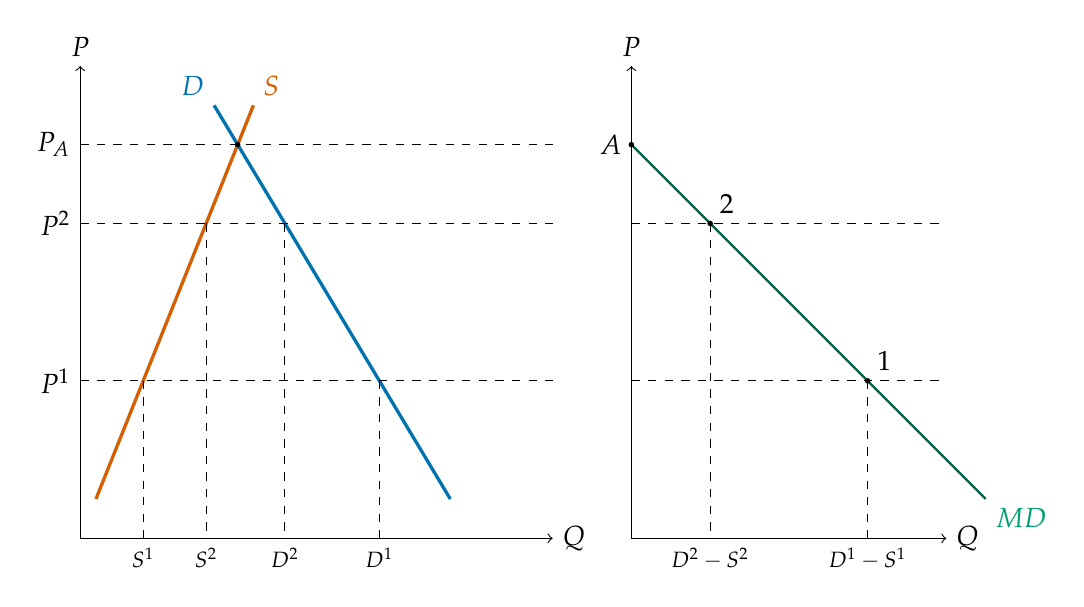
\begin{tikzpicture}[scale=0.5]

%---------------------------------------
% Home demand and supply & MD
%---------------------------------------
\pgfmathdeclarefunction{QdH}{1}{\pgfmathparse{10 - 0.6*#1}}  % D(P)
\pgfmathdeclarefunction{QsH}{1}{\pgfmathparse{0.4*#1}}       % S(P)
\pgfmathdeclarefunction{MD}{1}{\pgfmathparse{10 - #1}}       % MD(P)=D-S

%---------------------------------------
% Prices
%---------------------------------------
\def\Pmin{1}
\def\Pmax{11}
\def\PA{10}  % autarky price (Home)
\def\Pone{4}
\def\Ptwo{8}

%---------------------------------------
% Compute quantities at P^1 and P^2
%---------------------------------------
\pgfmathsetmacro{\QdOne}{10-0.6*\Pone}
\pgfmathsetmacro{\QsOne}{0.4*\Pone}
\pgfmathsetmacro{\MDOne}{\QdOne-\QsOne}

\pgfmathsetmacro{\QdTwo}{10-0.6*\Ptwo}
\pgfmathsetmacro{\QsTwo}{0.4*\Ptwo}
\pgfmathsetmacro{\MDTwo}{\QdTwo-\QsTwo}

% Autarky quantity
\pgfmathsetmacro{\Qaut}{10-0.6*\PA} % = 4

%---------------------------------------
% LEFT PANEL: Domestic S and D
%---------------------------------------
\begin{scope}[xshift=0cm]
  % Axes
  \draw[->] (0,0) -- (0,\Pmax+1) node[above] {$P$};
  \draw[->] (0,0) -- (12,0) node[right] {$Q$};

  % Demand curve
  \draw[very thick, blue, domain=\Pmin:\Pmax, samples=100] 
        plot ({QdH(\x)},{\x});
  \node[above left, blue] at ({QdH(\Pmax)},{\Pmax}) {$D$};

  % Supply curve
  \draw[very thick, red, domain=\Pmin:\Pmax, samples=100]
        plot ({QsH(\x)},{\x});
  \node[above right, red] at ({QsH(\Pmax)},{\Pmax}) {$S$};

  % Horizontal price lines
  \foreach \p/\lab in {\PA/P_A,\Ptwo/P^2,\Pone/P^1}{
    \draw[dashed] (0,\p) -- (12,\p);
    \node[left] at (0,\p) {$\lab$};
  }

  % Autarky intersection
  \fill (\Qaut,\PA) circle (2pt);

  % ---- Points at P^1 ----
  \draw[dashed] (\QdOne,\Pone) -- (\QdOne,0);
  \draw[dashed] (\QsOne,\Pone) -- (\QsOne,0);
  \node[below] at (\QdOne,0) {\footnotesize $D^1$};
  \node[below] at (\QsOne,0) {\footnotesize $S^1$};

  % ---- Points at P^2 ----
  \draw[dashed] (\QdTwo,\Ptwo) -- (\QdTwo,0);
  \draw[dashed] (\QsTwo,\Ptwo) -- (\QsTwo,0);
  \node[below] at (\QdTwo,0) {\footnotesize $D^2$};
  \node[below] at (\QsTwo,0) {\footnotesize $S^2$};

\end{scope}

%---------------------------------------
% RIGHT PANEL: Import demand MD(P)
%---------------------------------------
\begin{scope}[xshift=14cm]
  % Axes
  \draw[->] (0,0) -- (0,\Pmax+1) node[above] {$P$};
  \draw[->] (0,0) -- (8,0) node[right] {$Q$};

  % Import demand curve
  \draw[thick, green!60!black, domain=\Pmin:\PA, samples=100]
        plot ({MD(\x)},{\x});
  \node[below right, green] at ({MD(\Pmin)},{\Pmin}) {$MD$};

  % Autarky point A
  \fill (0,\PA) circle (2pt) node[left] {$A$};

  % Horizontal lines
  \draw[dashed] (0,\Ptwo) -- (8,\Ptwo);
  \draw[dashed] (0,\Pone) -- (8,\Pone);

  % ---- Point at P^2 ----
  \fill (\MDTwo,\Ptwo) circle (2pt) node[above right] {$2$};
  \draw[dashed] (\MDTwo,\Ptwo) -- (\MDTwo,0);
  \node[below] at (\MDTwo,0) {\footnotesize $D^2 - S^2$};

  % ---- Point at P^1 ----
  \fill (\MDOne,\Pone) circle (2pt) node[above right] {$1$};
  \draw[dashed] (\MDOne,\Pone) -- (\MDOne,0);
  \node[below] at (\MDOne,0) {\footnotesize $D^1 - S^1$};

\end{scope}

\end{tikzpicture}
\end{figure}
\end{frame}


\begin{frame}{Export supply}
\begin{wideitemize}
    \item At the \blue{foreign} country, we can define supply and demand curves as a function of prices:
    \item<2-> \blue{Foreign supply function} of a given good at prices $p$: $S^*(p)$
    \item<2-> \blue{Foreign demand function} of a given good at prices $p$: $D^*(p)$
    \item<3-> Assumptions:
    \begin{itemize}
        \item Supply slopes up ${S^*}'(p) > 0$
        \item Demand slopes down ${D^*}'(p) < 0$
    \end{itemize}
    \item<4-> Define the \textcolor{brown}{export supply} function:
    \begin{itemize}
        \item Export supply = foreign supply - foreign demand: $XS(p) = S^*(p) - D^*(p)$ 
    \end{itemize}
\end{wideitemize}
    
\end{frame}

\begin{frame}{Export supply: graphical representation}
\begin{figure}
\centering
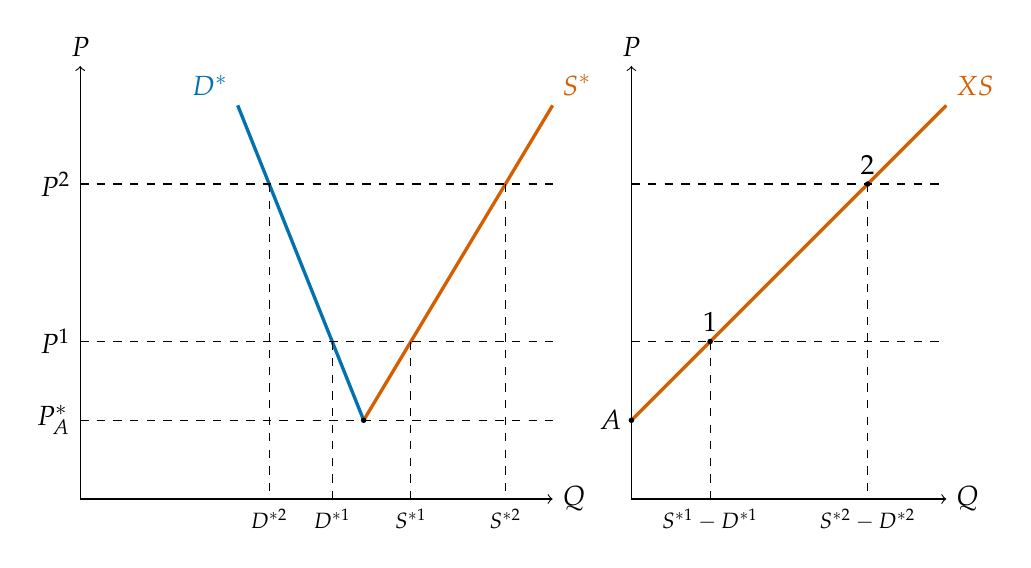
\begin{tikzpicture}[scale=0.5]

%---------------------------------------
% Foreign demand and supply & XS
%---------------------------------------
\pgfmathdeclarefunction{QdF}{1}{\pgfmathparse{8 - 0.4*#1}}   % D^*(P)
\pgfmathdeclarefunction{QsF}{1}{\pgfmathparse{6 + 0.6*#1}}   % S^*(P)
\pgfmathdeclarefunction{XS}{1}{\pgfmathparse{#1 - 2}}        % XS(P)=S*-D*

%---------------------------------------
% Prices
%---------------------------------------
\def\Pmin{2}
\def\Pmax{10}
\def\PA{2}   % foreign autarky price P_A^*
\def\Pone{4}
\def\Ptwo{8}

%---------------------------------------
% Compute quantities
%---------------------------------------
\pgfmathsetmacro{\QdOne}{8-0.4*\Pone}
\pgfmathsetmacro{\QsOne}{6+0.6*\Pone}
\pgfmathsetmacro{\XSOne}{\QsOne-\QdOne}

\pgfmathsetmacro{\QdTwo}{8-0.4*\Ptwo}
\pgfmathsetmacro{\QsTwo}{6+0.6*\Ptwo}
\pgfmathsetmacro{\XSTwo}{\QsTwo-\QdTwo}

\pgfmathsetmacro{\Qaut}{8-0.4*\PA} % = 7.2

%---------------------------------------
% LEFT PANEL: Foreign S* and D*
%---------------------------------------
\begin{scope}[xshift=0cm]
  % Axes
  \draw[->] (0,0) -- (0,\Pmax+1) node[above] {$P$};
  \draw[->] (0,0) -- (12,0) node[right] {$Q$};

  % D*
  \draw[very thick, blue, domain=\Pmin:\Pmax, samples=100]
        plot ({QdF(\x)},{\x});
  \node[above left, blue] at ({QdF(\Pmax)},\Pmax) {$D^*$};

  % S*
  \draw[very thick, red, domain=\Pmin:\Pmax, samples=100]
        plot ({QsF(\x)},{\x});
  \node[above right, red] at ({QsF(\Pmax)},\Pmax) {$S^*$};

  % Horizontal price lines
  \foreach \p/\lab in {\PA/P_A^*,\Pone/P^1,\Ptwo/P^2}{
    \draw[dashed] (0,\p) -- (12,\p);
    \node[left] at (0,\p) {$\lab$};
  }

  % Autarky
  \fill (\Qaut,\PA) circle (2pt);

  % P^1
  \draw[dashed] (\QdOne,\Pone) -- (\QdOne,0);
  \draw[dashed] (\QsOne,\Pone) -- (\QsOne,0);
  \node[below] at (\QdOne,0) {\footnotesize $D^{*1}$};
  \node[below] at (\QsOne,0) {\footnotesize $S^{*1}$};

  % P^2
  \draw[dashed] (\QdTwo,\Ptwo) -- (\QdTwo,0);
  \draw[dashed] (\QsTwo,\Ptwo) -- (\QsTwo,0);
  \node[below] at (\QdTwo,0) {\footnotesize $D^{*2}$};
  \node[below] at (\QsTwo,0) {\footnotesize $S^{*2}$};

\end{scope}

%---------------------------------------
% RIGHT PANEL: Export supply XS(P)
%---------------------------------------
\begin{scope}[xshift=14cm]
  % Axes
  \draw[->] (0,0) -- (0,\Pmax+1) node[above] {$P$};
  \draw[->] (0,0) -- (8,0) node[right] {$Q$};

  % XS curve
  \draw[very thick, red, domain=\PA:\Pmax, samples=100]
        plot ({XS(\x)},{\x});
  \node[above right, red] at ({XS(\Pmax)},\Pmax) {$XS$};

  % Autarky point
  \fill (0,\PA) circle (2pt) node[left] {$A$};

  % Horizontals
  \draw[dashed] (0,\Pone) -- (8,\Pone);
  \draw[dashed] (0,\Ptwo) -- (8,\Ptwo);

  % P^1
  \fill (\XSOne,\Pone) circle (2pt) node[above] {$1$};
  \draw[dashed] (\XSOne,\Pone) -- (\XSOne,0);
  \node[below] at (\XSOne,0) {\footnotesize $S^{*1} - D^{*1}$};

  % P^2
  \fill (\XSTwo,\Ptwo) circle (2pt) node[above] {$2$};
  \draw[dashed] (\XSTwo,\Ptwo) -- (\XSTwo,0);
  \node[below] at (\XSTwo,0) {\footnotesize $S^{*2} - D^{*2}$};

\end{scope}

\end{tikzpicture}
\end{figure}

\end{frame}

\begin{frame}{World equilibrium}
\begin{wideitemize}
    \item To find the equilibrium point, we must use a market clearing condition \\
    \qquad (which one?)
    \item<2-> In \blue{equilibrium}:
    \begin{eqnarray*}
    \text{Home demand - Home supply} &=& \text{Foreign supply - Foreign demand} \\
    \text{Home demand + Foreign demand} &=& \text{Home supply + Foreign supply} \\
    \text{World demand} &=& \text{World supply} \\
    \end{eqnarray*}
    \item<3-> More formally, equilibrium prices $P_W$ are those that satisfy:
    \begin{equation*}
        XS(P_W) = MD(P_W)
    \end{equation*}
\end{wideitemize}
    
\end{frame}


\begin{frame}{World equilibrium: graphical representation}
\begin{figure}
\centering
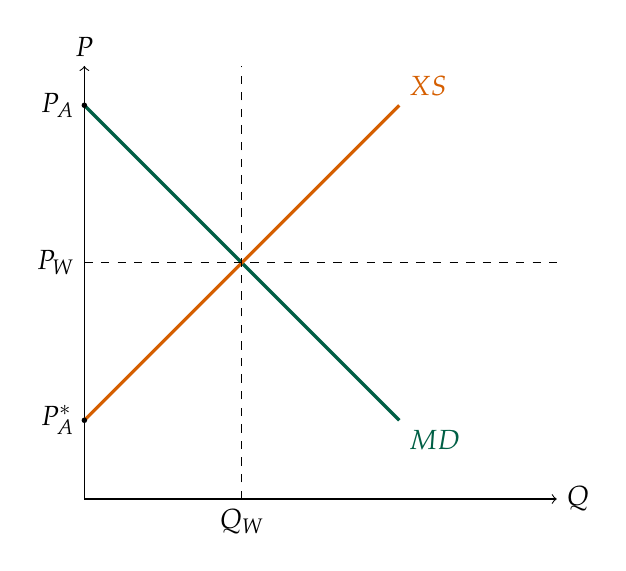
\begin{tikzpicture}[scale=0.5]

% World MD and XS
\pgfmathdeclarefunction{MD}{1}{\pgfmathparse{10 - #1}}  % MD(P)
\pgfmathdeclarefunction{XS}{1}{\pgfmathparse{#1 - 2}}   % XS(P)

\def\PAH{10}  % Home autarky P_A
\def\PAF{2}   % Foreign autarky P_A^*
\def\Pmin{2}
\def\Pmax{10}

\pgfmathsetmacro{\Pw}{6}
\pgfmathsetmacro{\Qw}{10-\Pw}  % =4

% Axes
\draw[->] (0,0) -- (0,\Pmax+1) node[above] {$P$};
\draw[->] (0,0) -- (12,0) node[right] {$Q$};

% MD curve
\draw[very thick, green!60!black, domain=\PAF:\PAH, samples=100]
    plot ({MD(\x)},{\x});
\node[below right, green!60!black] at ({MD(\Pmin)},{\Pmin}) {$MD$};

% XS curve
\draw[very thick, red, domain=\PAF:\PAH, samples=100]
    plot ({XS(\x)},{\x});
\node[above right, red] at ({XS(\Pmax)},{\Pmax}) {$XS$};

% Autarky prices
\fill (0,\PAH) circle (2pt) node[left] {$P_A$};
\fill (0,\PAF) circle (2pt) node[left] {$P_A^*$};

% Dashed lines
\draw[dashed] (0,\Pw) -- (12,\Pw);
\draw[dashed] (\Qw,0) -- (\Qw,\Pmax+1);

\node[left]  at (0,\Pw) {$P_W$};
\node[below] at (\Qw,0) {$Q_W$};

\end{tikzpicture}
\end{figure}
\end{frame}


\begin{frame}{World Equilibrium: graphical representation (ii)}
\begin{figure}
\centering
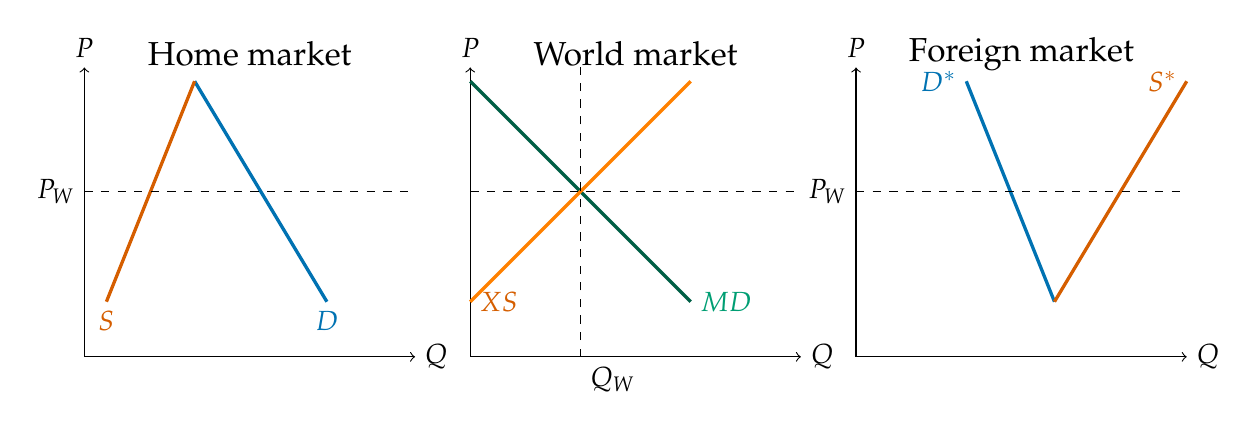
\begin{tikzpicture}[scale=0.35]

%---------------------------------------
% Shared functions
%---------------------------------------
\pgfmathdeclarefunction{QdH}{1}{\pgfmathparse{10 - 0.6*#1}}  % Home D
\pgfmathdeclarefunction{QsH}{1}{\pgfmathparse{0.4*#1}}       % Home S
\pgfmathdeclarefunction{QdF}{1}{\pgfmathparse{8 - 0.4*#1}}   % Foreign D*
\pgfmathdeclarefunction{QsF}{1}{\pgfmathparse{6 + 0.6*#1}}   % Foreign S*
\pgfmathdeclarefunction{MD}{1}{\pgfmathparse{10 - #1}}       % MD
\pgfmathdeclarefunction{XS}{1}{\pgfmathparse{#1 - 2}}        % XS

\def\Pmin{2}
\def\Pmax{10}

% World equilibrium & tariff
\def\Pw{6}
\def\Qw{4}

\def\Qt{3}
\def\PT{7}
\def\PTstar{5}
\def\twedge{2}

%====================================================
% LEFT PANEL: Home market
%====================================================
\begin{scope}[xshift=0cm]
  \node at (6,\Pmax+1) {\large Home market};

  % Axes
  \draw[->] (0,0) -- (0,\Pmax+0.5) node[above] {$P$};
  \draw[->] (0,0) -- (12,0) node[right] {$Q$};

  % Home demand and supply (true functional forms)
  \draw[very thick, blue, domain=\Pmin:\Pmax, samples=100]
        plot ({QdH(\x)},{\x});
  \draw[very thick, red, domain=\Pmin:\Pmax, samples=100]
        plot ({QsH(\x)},{\x});

  \node[below, blue] at ({QdH(\Pmin)},\Pmin) {$D$};
  \node[below, red]  at ({QsH(\Pmin)},\Pmin) {$S$};

  % Prices PW and PT
  \draw[dashed] (0,\Pw) -- (12,\Pw);

  \node[left] at (0,\Pw) {$P_W$};
\end{scope}

%====================================================
% MIDDLE PANEL: World market (MD and XS)
%====================================================
\begin{scope}[xshift=14cm]
  \node at (6,\Pmax+1) {\large World market};

  % Axes
  \draw[->] (0,0) -- (0,\Pmax+0.5) node[above] {$P$};
  \draw[->] (0,0) -- (12,0) node[right] {$Q$};

  % MD and XS
  \draw[very thick, green!60!black, domain=\Pmin:\Pmax, samples=100]
      plot ({MD(\x)},{\x});
  \node[right, green] at ({MD(\Pmin)},{\Pmin}) {$MD$};
  \draw[very thick, orange, domain=\Pmin:\Pmax, samples=100]
      plot ({XS(\x)},{\x});
  \node[right, red] at ({XS(\Pmin)},{\Pmin}) {$XS$};

  % Vertical line at Q_W
  \draw[dashed] (\Qw,0) -- (\Qw,\Pmax+0.5);
  \node[below right] at (\Qw,0) {$Q_W$};

  % Horizontal lines for P_T, P_W, P_T^*
  \draw[dashed] (0,\Pw) -- (12,\Pw);

\end{scope}

%====================================================
% RIGHT PANEL: Foreign market
%====================================================
\begin{scope}[xshift=28cm]
  \node at (6,\Pmax+1) {\large Foreign market};

  % Axes
  \draw[->] (0,0) -- (0,\Pmax+0.5) node[above] {$P$};
  \draw[->] (0,0) -- (12,0) node[right] {$Q$};

  % Foreign demand and supply
  \draw[very thick, blue, domain=\Pmin:\Pmax, samples=100]
        plot ({QdF(\x)},{\x});
  \draw[very thick, red, domain=\Pmin:\Pmax, samples=100]
        plot ({QsF(\x)},{\x});

  \node[blue, left] at ({QdF(\Pmax)},\Pmax) {$D^*$};
  \node[red, left]  at ({QsF(\Pmax)},\Pmax) {$S^*$};

  % Prices P_W and P_T^*
  \draw[dashed] (0,\Pw) -- (12,\Pw);

  \node[left] at (0,\Pw) {$P_W$};
\end{scope}

\end{tikzpicture}
\end{figure}
\end{frame}

\begin{frame}{Tariffs}
\begin{wideitemize}
    \item Tariffs are import taxes
    \item<2-> Tariffs are wedges (gaps) between the source country and the destination country prices:
    \begin{itemize}
        \item \blue{Simple tariffs}: $P = P^* + t$, where $t$ is some dollar amount \\
        \qquad (used, e.g., for imports of alcohol and tobacco; more common back in the day)
        \item \blue{Ad valorem tariffs}: $P = P^*(1+\tau)$, where $\tau$ is some percentage \\
        \qquad (used for most goods currently)
    \end{itemize}
    \item<3-> Who pays for the tariffs?
    \begin{itemize}
        \item<4-> In an \blue{accounting} sense, importing firms
        \item<5-> In an \blue{economic} sense, it depends on supply and demand elasticity
    \end{itemize}
\end{wideitemize}
    
\end{frame}


\begin{frame}{Effects of a Tariff in a small country}
\begin{figure}
\centering
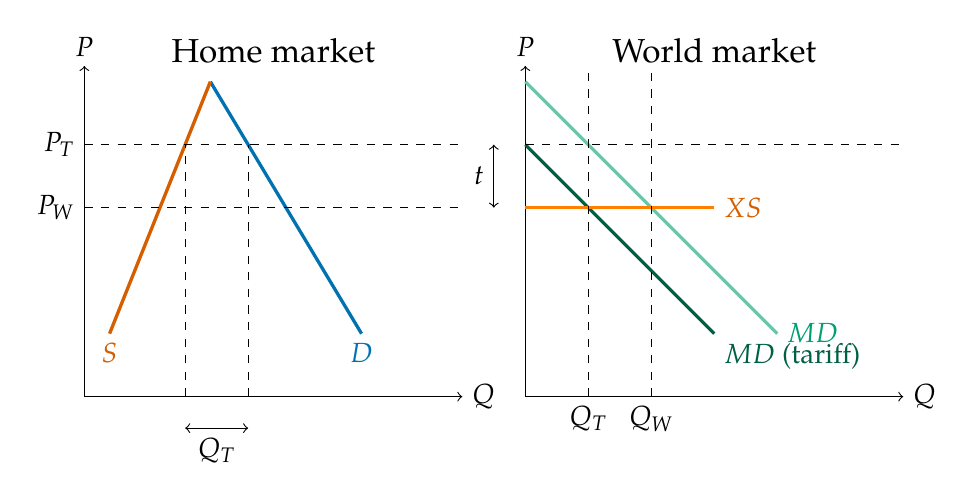
\begin{tikzpicture}[scale=0.4]

%---------------------------------------
% Shared functions
%---------------------------------------
\pgfmathdeclarefunction{QdH}{1}{\pgfmathparse{10 - 0.6*#1}}  % Home D
\pgfmathdeclarefunction{QsH}{1}{\pgfmathparse{0.4*#1}}       % Home S
\pgfmathdeclarefunction{QdF}{1}{\pgfmathparse{8 - 0.4*#1}}   % Foreign D*
\pgfmathdeclarefunction{QsF}{1}{\pgfmathparse{6 + 0.6*#1}}   % Foreign S*
\pgfmathdeclarefunction{MD}{1}{\pgfmathparse{10 - #1}}       % MD
\pgfmathdeclarefunction{MDt}{1}{\pgfmathparse{8 - #1}}       % MD
\pgfmathdeclarefunction{XS}{1}{\pgfmathparse{6}}        % XS

\def\Pmin{2}
\def\Pmax{10}

% World equilibrium & tariff
\def\Pw{6}
\def\Qw{4}

\def\PT{8}
\def\Qt{{MD(\PT)}}
\def\twedge{2}

%====================================================
% LEFT PANEL: Home market
%====================================================
\begin{scope}[xshift=0cm]
  \node at (6,\Pmax+1) {\large Home market};

  % Axes
  \draw[->] (0,0) -- (0,\Pmax+0.5) node[above] {$P$};
  \draw[->] (0,0) -- (12,0) node[right] {$Q$};

  % Home demand and supply (true functional forms)
  \draw[very thick, blue, domain=\Pmin:\Pmax, samples=100]
        plot ({QdH(\x)},{\x});
  \draw[very thick, red, domain=\Pmin:\Pmax, samples=100]
        plot ({QsH(\x)},{\x});

  \node[below, blue] at ({QdH(\Pmin)},\Pmin) {$D$};
  \node[below, red]  at ({QsH(\Pmin)},\Pmin) {$S$};

  \draw[dashed] ({QsH(\PT)},0) -- ({QsH(\PT)},\PT);
  \draw[dashed] ({QdH(\PT)},0) -- ({QdH(\PT)},\PT);
  \draw[<->] ({QsH(\PT)},-1) -- ({QdH(\PT)},-1)
      node[midway,below] {$Q_T$};
  % Prices PW and PT
  \draw[dashed] (0,\Pw) -- (12,\Pw);
  \draw[dashed] (0,\PT) -- (12,\PT);

  \node[left] at (0,\Pw) {$P_W$};
  \node[left] at (0,\PT) {$P_T$};
\end{scope}

%====================================================
% MIDDLE PANEL: World market (MD and XS)
%====================================================
\begin{scope}[xshift=14cm]
  \node at (6,\Pmax+1) {\large World market};

  % Axes
  \draw[->] (0,0) -- (0,\Pmax+0.5) node[above] {$P$};
  \draw[->] (0,0) -- (12,0) node[right] {$Q$};

  % MD and XS
  \draw[very thick, green!60, domain=\Pmin:\Pmax, samples=100]
      plot ({MD(\x)},{\x});
  \node[right, green] at ({MD(\Pmin)},{\Pmin}) {$MD$};
  \draw[very thick, green!60!black, domain=\Pmin:\Pmax-2, samples=100]
      plot ({MDt(\x)},{\x});
  \node[below right, green!60!black] at ({MDt(\Pmin)},{\Pmin}) {$MD$ (tariff)};
  \draw[very thick, orange] (0,\Pw) -- ({XS(\Pmax)},\Pw);
  \node[right, red] at ({XS(\Pmax)},\Pw) {$XS$};

  % New quantity with tariff Q_T
  \draw[dashed] (\Qt,0) -- (\Qt,\Pmax+0.5);
  \node[below] at (\Qt,0) {$Q_T$};



  % Vertical line at Q_W
  \draw[dashed] (\Qw,0) -- (\Qw,\Pmax+0.5);
  \node[below] at (\Qw,0) {$Q_W$};

  % Horizontal lines for P_T, P_W, P_T^*
  \draw[dashed] (0,\PT) -- (12,\PT);

  % Tariff wedge t = P_T - P_T^*
  \draw[<->] (-1,\PT) -- (-1,\Pw)
      node[midway,left] {$t$};
\end{scope}

\end{tikzpicture}
\end{figure}
\end{frame}

\begin{frame}{Effects of a Tariff in a small country: discussion}
\begin{wideitemize}
    \item In a small country, \blue{domestic import demand does not impact global markets}

    \item<2-> World price $P_W$ not only taken as given, but \blue{unaffected by import demand}

    \item<3-> \textcolor{brown}{Export supply curve (XS)} is infinitely elastic, meaning foreign producers :
    \begin{itemize}
        \item supply \textbf{any} volume of exports at the world price $P_W$, but...
        \item ...supply \textbf{zero} exports at a price below $P_W$
        \item ...supply \textbf{infinite} exports at a price above $P_W$ 
    \end{itemize}
    \item<4-> \blue{Intuition}: flexible production, constant costs, tiny price change $\rightarrow$ massive change in quantity supplied.
    \item<5-> In that case, tariffs are fully passed through to domestic market: $P = P_W + t$
    \item<6-> Reduces imports to $Q_T < Q_W$
\end{wideitemize}
\end{frame}

\begin{frame}{Welfare effects of a Tariff in a small country}
\begin{figure}
\centering
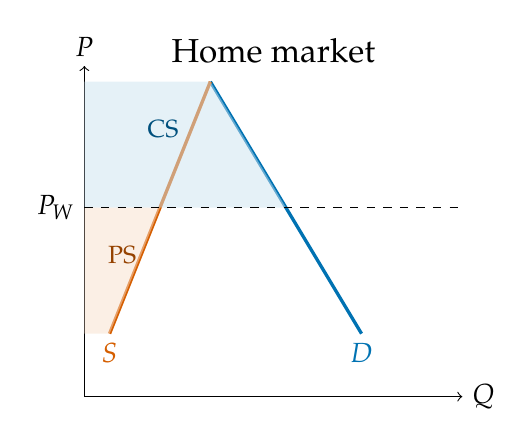
\begin{tikzpicture}[scale=0.4]

%---------------------------------------
% Shared functions
%---------------------------------------
\pgfmathdeclarefunction{QdH}{1}{\pgfmathparse{10 - 0.6*#1}}  % Home D
\pgfmathdeclarefunction{QsH}{1}{\pgfmathparse{0.4*#1}}       % Home S
\pgfmathdeclarefunction{QdF}{1}{\pgfmathparse{8 - 0.4*#1}}   % Foreign D*
\pgfmathdeclarefunction{QsF}{1}{\pgfmathparse{6 + 0.6*#1}}   % Foreign S*
\pgfmathdeclarefunction{MD}{1}{\pgfmathparse{10 - #1}}       % MD
\pgfmathdeclarefunction{XS}{1}{\pgfmathparse{6}}             % XS

\def\Pmin{2}
\def\Pmax{10}

% World equilibrium & tariff
\def\Pw{6}
\def\Qw{4}

\def\PT{8}
\def\Qt{{MD(\PT)}}
\def\twedge{2}

%====================================================
% LEFT PANEL: Home market
%====================================================
\begin{scope}[xshift=0cm]
  \node at (6,\Pmax+1) {\large Home market};

  % Axes
  \draw[->] (0,0) -- (0,\Pmax+0.5) node[above] {$P$};
  \draw[->] (0,0) -- (12,0) node[right] {$Q$};

  % Home demand and supply (true functional forms)
  \draw[very thick, blue, domain=\Pmin:\Pmax, samples=100]
        plot ({QdH(\x)},{\x});
  \draw[very thick, red, domain=\Pmin:\Pmax, samples=100]
        plot ({QsH(\x)},{\x});

  \node[below, blue] at ({QdH(\Pmin)},\Pmin) {$D$};
  \node[below, red]  at ({QsH(\Pmin)},\Pmin) {$S$};

  % ---- Consumer surplus (under D, above P_W) ----
  \fill[blue!20, opacity=0.5]
    (0,\Pw)
    -- ({QdH(\Pw)},\Pw)
    -- ({QdH(\Pmax)},\Pmax)
    -- (0,\Pmax)
    -- cycle;

  % Label CS
  \node[blue!70!black] at (2.5,8.5) {\small CS};

  % ---- Producer surplus (above S, below P_W) ----
  \fill[red!20, opacity=0.5]
    (0,\Pmin)
    -- (0,\Pw)
    -- ({QsH(\Pw)},\Pw)
    -- ({QsH(\Pmin)},\Pmin)
    -- (0,\Pmin)
    -- cycle;

  % Label PS
  \node[red!70!black] at (1.2,4.5) {\small PS};

  % World price line P_W
  \draw[dashed] (0,\Pw) -- (12,\Pw);
  \node[left] at (0,\Pw) {$P_W$};

\end{scope}

\end{tikzpicture}
\end{figure}

\end{frame}


\begin{frame}{Welfare effects of a Tariff in a small country}
\addtocounter{framenumber}{-1}
\begin{figure}
\centering
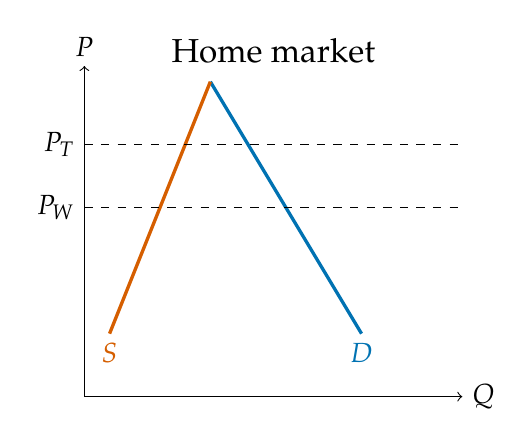
\begin{tikzpicture}[scale=0.4]

%---------------------------------------
% Shared functions
%---------------------------------------
\pgfmathdeclarefunction{QdH}{1}{\pgfmathparse{10 - 0.6*#1}}  % Home D
\pgfmathdeclarefunction{QsH}{1}{\pgfmathparse{0.4*#1}}       % Home S
\pgfmathdeclarefunction{QdF}{1}{\pgfmathparse{8 - 0.4*#1}}   % Foreign D*
\pgfmathdeclarefunction{QsF}{1}{\pgfmathparse{6 + 0.6*#1}}   % Foreign S*
\pgfmathdeclarefunction{MD}{1}{\pgfmathparse{10 - #1}}       % MD
\pgfmathdeclarefunction{XS}{1}{\pgfmathparse{6}}        % XS

\def\Pmin{2}
\def\Pmax{10}

% World equilibrium & tariff
\def\Pw{6}
\def\Qw{4}

\def\PT{8}
\def\Qt{{MD(\PT)}}
\def\twedge{2}

%====================================================
% LEFT PANEL: Home market
%====================================================
\begin{scope}[xshift=0cm]
  \node at (6,\Pmax+1) {\large Home market};

  % Axes
  \draw[->] (0,0) -- (0,\Pmax+0.5) node[above] {$P$};
  \draw[->] (0,0) -- (12,0) node[right] {$Q$};

  % Home demand and supply (true functional forms)
  \draw[very thick, blue, domain=\Pmin:\Pmax, samples=100]
        plot ({QdH(\x)},{\x});
  \draw[very thick, red, domain=\Pmin:\Pmax, samples=100]
        plot ({QsH(\x)},{\x});

  \node[below, blue] at ({QdH(\Pmin)},\Pmin) {$D$};
  \node[below, red]  at ({QsH(\Pmin)},\Pmin) {$S$};

  % Prices PW and PT
  \draw[dashed] (0,\Pw) -- (12,\Pw);
  \draw[dashed] (0,\PT) -- (12,\PT);

  \node[left] at (0,\Pw) {$P_W$};
  \node[left] at (0,\PT) {$P_T$};
\end{scope}



\end{tikzpicture}
\end{figure}

\end{frame}

\begin{frame}{Welfare effects of a Tariff in a small country}
\addtocounter{framenumber}{-1}
\begin{figure}
\centering
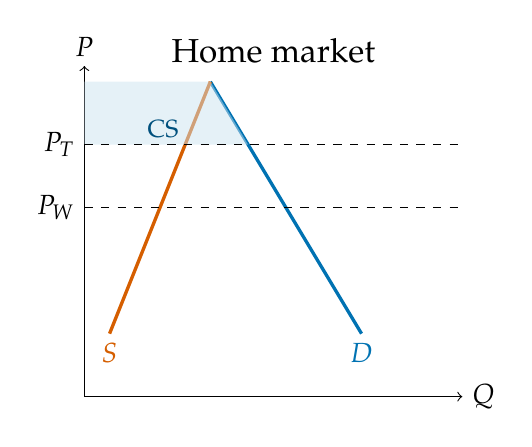
\begin{tikzpicture}[scale=0.4]

%---------------------------------------
% Shared functions
%---------------------------------------
\pgfmathdeclarefunction{QdH}{1}{\pgfmathparse{10 - 0.6*#1}}  % Home D
\pgfmathdeclarefunction{QsH}{1}{\pgfmathparse{0.4*#1}}       % Home S
\pgfmathdeclarefunction{QdF}{1}{\pgfmathparse{8 - 0.4*#1}}   % Foreign D*
\pgfmathdeclarefunction{QsF}{1}{\pgfmathparse{6 + 0.6*#1}}   % Foreign S*
\pgfmathdeclarefunction{MD}{1}{\pgfmathparse{10 - #1}}       % MD
\pgfmathdeclarefunction{XS}{1}{\pgfmathparse{6}}        % XS

\def\Pmin{2}
\def\Pmax{10}

% World equilibrium & tariff
\def\Pw{6}
\def\Qw{4}

\def\PT{8}
\def\Qt{{MD(\PT)}}
\def\twedge{2}

%====================================================
% LEFT PANEL: Home market
%====================================================
\begin{scope}[xshift=0cm]
  \node at (6,\Pmax+1) {\large Home market};

  % Axes
  \draw[->] (0,0) -- (0,\Pmax+0.5) node[above] {$P$};
  \draw[->] (0,0) -- (12,0) node[right] {$Q$};

  % Home demand and supply (true functional forms)
  \draw[very thick, blue, domain=\Pmin:\Pmax, samples=100]
        plot ({QdH(\x)},{\x});
  \draw[very thick, red, domain=\Pmin:\Pmax, samples=100]
        plot ({QsH(\x)},{\x});

  \node[below, blue] at ({QdH(\Pmin)},\Pmin) {$D$};
  \node[below, red]  at ({QsH(\Pmin)},\Pmin) {$S$};

  % ---- Consumer surplus (under D, above P_W) ----
  \fill[blue!20, opacity=0.5]
    (0,\PT)
    -- ({QdH(\PT)},\PT)
    -- ({QdH(\Pmax)},\Pmax)
    -- (0,\Pmax)
    -- cycle;

  % Label CS
  \node[blue!70!black] at (2.5,8.5) {\small CS};


  % Prices PW and PT
  \draw[dashed] (0,\Pw) -- (12,\Pw);
  \draw[dashed] (0,\PT) -- (12,\PT);

  \node[left] at (0,\Pw) {$P_W$};
  \node[left] at (0,\PT) {$P_T$};
\end{scope}



\end{tikzpicture}
\end{figure}

\end{frame}


\begin{frame}{Welfare effects of a Tariff in a small country}
\addtocounter{framenumber}{-1}
\begin{figure}
\centering
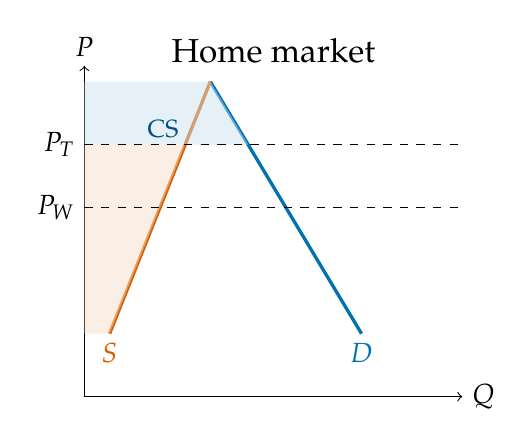
\begin{tikzpicture}[scale=0.4]

%---------------------------------------
% Shared functions
%---------------------------------------
\pgfmathdeclarefunction{QdH}{1}{\pgfmathparse{10 - 0.6*#1}}  % Home D
\pgfmathdeclarefunction{QsH}{1}{\pgfmathparse{0.4*#1}}       % Home S
\pgfmathdeclarefunction{QdF}{1}{\pgfmathparse{8 - 0.4*#1}}   % Foreign D*
\pgfmathdeclarefunction{QsF}{1}{\pgfmathparse{6 + 0.6*#1}}   % Foreign S*
\pgfmathdeclarefunction{MD}{1}{\pgfmathparse{10 - #1}}       % MD
\pgfmathdeclarefunction{XS}{1}{\pgfmathparse{6}}        % XS

\def\Pmin{2}
\def\Pmax{10}

% World equilibrium & tariff
\def\Pw{6}
\def\Qw{4}

\def\PT{8}
\def\Qt{{MD(\PT)}}
\def\twedge{2}

%====================================================
% LEFT PANEL: Home market
%====================================================
\begin{scope}[xshift=0cm]
  \node at (6,\Pmax+1) {\large Home market};

  % Axes
  \draw[->] (0,0) -- (0,\Pmax+0.5) node[above] {$P$};
  \draw[->] (0,0) -- (12,0) node[right] {$Q$};

  % Home demand and supply (true functional forms)
  \draw[very thick, blue, domain=\Pmin:\Pmax, samples=100]
        plot ({QdH(\x)},{\x});
  \draw[very thick, red, domain=\Pmin:\Pmax, samples=100]
        plot ({QsH(\x)},{\x});

  \node[below, blue] at ({QdH(\Pmin)},\Pmin) {$D$};
  \node[below, red]  at ({QsH(\Pmin)},\Pmin) {$S$};

  % ---- Consumer surplus (under D, above P_W) ----
  \fill[blue!20, opacity=0.5]
    (0,\PT)
    -- ({QdH(\PT)},\PT)
    -- ({QdH(\Pmax)},\Pmax)
    -- (0,\Pmax)
    -- cycle;

  % Label CS
  \node[blue!70!black] at (2.5,8.5) {\small CS};

  % ---- Producer surplus (above S, below P_W) ----
  \fill[red!20, opacity=0.5]
    (0,\Pmin)
    -- (0,\PT)
    -- ({QsH(\PT)},\PT)
    -- ({QsH(\Pmin)},\Pmin)
    -- (0,\Pmin)
    -- cycle;

  % Prices PW and PT
  \draw[dashed] (0,\Pw) -- (12,\Pw);
  \draw[dashed] (0,\PT) -- (12,\PT);

  \node[left] at (0,\Pw) {$P_W$};
  \node[left] at (0,\PT) {$P_T$};
\end{scope}



\end{tikzpicture}
\end{figure}

\end{frame}



\begin{frame}{Welfare effects of a Tariff in a small country}
\addtocounter{framenumber}{-1}
\begin{figure}
\centering
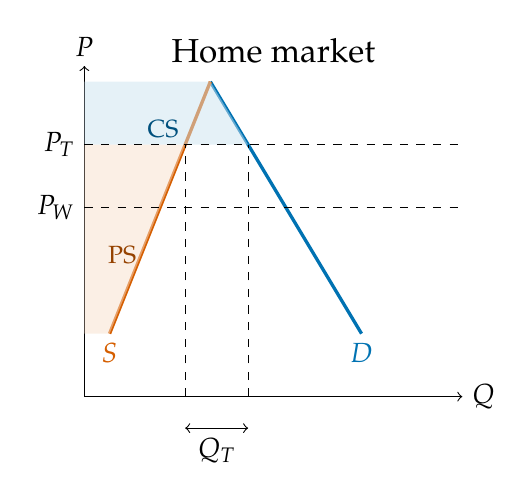
\begin{tikzpicture}[scale=0.4]

%---------------------------------------
% Shared functions
%---------------------------------------
\pgfmathdeclarefunction{QdH}{1}{\pgfmathparse{10 - 0.6*#1}}  % Home D
\pgfmathdeclarefunction{QsH}{1}{\pgfmathparse{0.4*#1}}       % Home S
\pgfmathdeclarefunction{QdF}{1}{\pgfmathparse{8 - 0.4*#1}}   % Foreign D*
\pgfmathdeclarefunction{QsF}{1}{\pgfmathparse{6 + 0.6*#1}}   % Foreign S*
\pgfmathdeclarefunction{MD}{1}{\pgfmathparse{10 - #1}}       % MD
\pgfmathdeclarefunction{XS}{1}{\pgfmathparse{6}}        % XS

\def\Pmin{2}
\def\Pmax{10}

% World equilibrium & tariff
\def\Pw{6}
\def\Qw{4}

\def\PT{8}
\def\Qt{{MD(\PT)}}
\def\twedge{2}

%====================================================
% LEFT PANEL: Home market
%====================================================
\begin{scope}[xshift=0cm]
  \node at (6,\Pmax+1) {\large Home market};

  % Axes
  \draw[->] (0,0) -- (0,\Pmax+0.5) node[above] {$P$};
  \draw[->] (0,0) -- (12,0) node[right] {$Q$};

  % Home demand and supply (true functional forms)
  \draw[very thick, blue, domain=\Pmin:\Pmax, samples=100]
        plot ({QdH(\x)},{\x});
  \draw[very thick, red, domain=\Pmin:\Pmax, samples=100]
        plot ({QsH(\x)},{\x});

  \node[below, blue] at ({QdH(\Pmin)},\Pmin) {$D$};
  \node[below, red]  at ({QsH(\Pmin)},\Pmin) {$S$};

  % ---- Consumer surplus (under D, above P_W) ----
  \fill[blue!20, opacity=0.5]
    (0,\PT)
    -- ({QdH(\PT)},\PT)
    -- ({QdH(\Pmax)},\Pmax)
    -- (0,\Pmax)
    -- cycle;

  % Label CS
  \node[blue!70!black] at (2.5,8.5) {\small CS};

  % ---- Producer surplus (above S, below P_W) ----
  \fill[red!20, opacity=0.5]
    (0,\Pmin)
    -- (0,\PT)
    -- ({QsH(\PT)},\PT)
    -- ({QsH(\Pmin)},\Pmin)
    -- (0,\Pmin)
    -- cycle;

  % Label PS
  \node[red!70!black] at (1.2,4.5) {\small PS};

  \draw[dashed] ({QsH(\PT)},0) -- ({QsH(\PT)},\PT);
  \draw[dashed] ({QdH(\PT)},0) -- ({QdH(\PT)},\PT);
  \draw[<->] ({QsH(\PT)},-1) -- ({QdH(\PT)},-1)
      node[midway,below] {$Q_T$};
  % Prices PW and PT
  \draw[dashed] (0,\Pw) -- (12,\Pw);
  \draw[dashed] (0,\PT) -- (12,\PT);

  \node[left] at (0,\Pw) {$P_W$};
  \node[left] at (0,\PT) {$P_T$};
\end{scope}



\end{tikzpicture}
\end{figure}

\end{frame}


\begin{frame}{Welfare effects of a Tariff in a small country}
\addtocounter{framenumber}{-1}
\begin{figure}
\centering
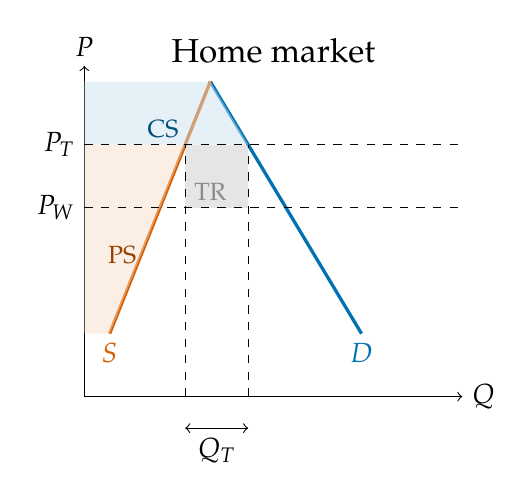
\begin{tikzpicture}[scale=0.4]

%---------------------------------------
% Shared functions
%---------------------------------------
\pgfmathdeclarefunction{QdH}{1}{\pgfmathparse{10 - 0.6*#1}}  % Home D
\pgfmathdeclarefunction{QsH}{1}{\pgfmathparse{0.4*#1}}       % Home S
\pgfmathdeclarefunction{QdF}{1}{\pgfmathparse{8 - 0.4*#1}}   % Foreign D*
\pgfmathdeclarefunction{QsF}{1}{\pgfmathparse{6 + 0.6*#1}}   % Foreign S*
\pgfmathdeclarefunction{MD}{1}{\pgfmathparse{10 - #1}}       % MD
\pgfmathdeclarefunction{XS}{1}{\pgfmathparse{6}}        % XS

\def\Pmin{2}
\def\Pmax{10}

% World equilibrium & tariff
\def\Pw{6}
\def\Qw{4}

\def\PT{8}
\def\Qt{{MD(\PT)}}
\def\twedge{2}

%====================================================
% LEFT PANEL: Home market
%====================================================
\begin{scope}[xshift=0cm]
  \node at (6,\Pmax+1) {\large Home market};

  % Axes
  \draw[->] (0,0) -- (0,\Pmax+0.5) node[above] {$P$};
  \draw[->] (0,0) -- (12,0) node[right] {$Q$};

  % Home demand and supply (true functional forms)
  \draw[very thick, blue, domain=\Pmin:\Pmax, samples=100]
        plot ({QdH(\x)},{\x});
  \draw[very thick, red, domain=\Pmin:\Pmax, samples=100]
        plot ({QsH(\x)},{\x});

  \node[below, blue] at ({QdH(\Pmin)},\Pmin) {$D$};
  \node[below, red]  at ({QsH(\Pmin)},\Pmin) {$S$};

  % ---- Consumer surplus (under D, above P_W) ----
  \fill[blue!20, opacity=0.5]
    (0,\PT)
    -- ({QdH(\PT)},\PT)
    -- ({QdH(\Pmax)},\Pmax)
    -- (0,\Pmax)
    -- cycle;

  % Label CS
  \node[blue!70!black] at (2.5,8.5) {\small CS};

  % ---- Producer surplus (above S, below P_W) ----
  \fill[red!20, opacity=0.5]
    (0,\Pmin)
    -- (0,\PT)
    -- ({QsH(\PT)},\PT)
    -- ({QsH(\Pmin)},\Pmin)
    -- (0,\Pmin)
    -- cycle;

  % Label TR
  \node[black!70] at (4,6.5) {\small TR};

  % ---- Tax Revenue ----
  \fill[black!20, opacity=0.5]
    ({QsH(\PT)},\PT)
    -- ({QdH(\PT)},\PT)
    -- ({QdH(\PT)},\Pw)
    -- ({QsH(\PT)},\Pw)
    -- cycle;

    
  % Label PS
  \node[red!70!black] at (1.2,4.5) {\small PS};

  \draw[dashed] ({QsH(\PT)},0) -- ({QsH(\PT)},\PT);
  \draw[dashed] ({QdH(\PT)},0) -- ({QdH(\PT)},\PT);
  \draw[<->] ({QsH(\PT)},-1) -- ({QdH(\PT)},-1)
      node[midway,below] {$Q_T$};
  % Prices PW and PT
  \draw[dashed] (0,\Pw) -- (12,\Pw);
  \draw[dashed] (0,\PT) -- (12,\PT);

  \node[left] at (0,\Pw) {$P_W$};
  \node[left] at (0,\PT) {$P_T$};
\end{scope}



\end{tikzpicture}
\end{figure}

\end{frame}

\begin{frame}{Welfare effects of a Tariff in a small country}
\addtocounter{framenumber}{-1}
\begin{figure}
\centering
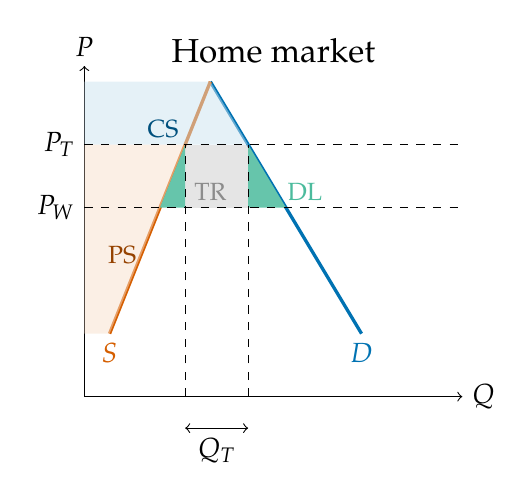
\begin{tikzpicture}[scale=0.4]

%---------------------------------------
% Shared functions
%---------------------------------------
\pgfmathdeclarefunction{QdH}{1}{\pgfmathparse{10 - 0.6*#1}}  % Home D
\pgfmathdeclarefunction{QsH}{1}{\pgfmathparse{0.4*#1}}       % Home S
\pgfmathdeclarefunction{QdF}{1}{\pgfmathparse{8 - 0.4*#1}}   % Foreign D*
\pgfmathdeclarefunction{QsF}{1}{\pgfmathparse{6 + 0.6*#1}}   % Foreign S*
\pgfmathdeclarefunction{MD}{1}{\pgfmathparse{10 - #1}}       % MD
\pgfmathdeclarefunction{XS}{1}{\pgfmathparse{6}}        % XS

\def\Pmin{2}
\def\Pmax{10}

% World equilibrium & tariff
\def\Pw{6}
\def\Qw{4}

\def\PT{8}
\def\Qt{{MD(\PT)}}
\def\twedge{2}

%====================================================
% LEFT PANEL: Home market
%====================================================
\begin{scope}[xshift=0cm]
  \node at (6,\Pmax+1) {\large Home market};

  % Axes
  \draw[->] (0,0) -- (0,\Pmax+0.5) node[above] {$P$};
  \draw[->] (0,0) -- (12,0) node[right] {$Q$};

  % Home demand and supply (true functional forms)
  \draw[very thick, blue, domain=\Pmin:\Pmax, samples=100]
        plot ({QdH(\x)},{\x});
  \draw[very thick, red, domain=\Pmin:\Pmax, samples=100]
        plot ({QsH(\x)},{\x});

  \node[below, blue] at ({QdH(\Pmin)},\Pmin) {$D$};
  \node[below, red]  at ({QsH(\Pmin)},\Pmin) {$S$};

  % ---- Consumer surplus (under D, above P_W) ----
  \fill[blue!20, opacity=0.5]
    (0,\PT)
    -- ({QdH(\PT)},\PT)
    -- ({QdH(\Pmax)},\Pmax)
    -- (0,\Pmax)
    -- cycle;

  % Label CS
  \node[blue!70!black] at (2.5,8.5) {\small CS};

  % ---- Producer surplus (above S, below P_W) ----
  \fill[red!20, opacity=0.5]
    (0,\Pmin)
    -- (0,\PT)
    -- ({QsH(\PT)},\PT)
    -- ({QsH(\Pmin)},\Pmin)
    -- (0,\Pmin)
    -- cycle;

  % Label TR
  \node[black!70] at (4,6.5) {\small TR};

  % ---- Tax Revenue ----
  \fill[black!20, opacity=0.5]
    ({QsH(\PT)},\PT)
    -- ({QdH(\PT)},\PT)
    -- ({QdH(\PT)},\Pw)
    -- ({QsH(\PT)},\Pw)
    -- cycle;

  % Label DL
  \node[green!70] at (7,6.5) {\small DL};

  % ---- Tax Deadweight Loss ----
  \fill[green!60, opacity=1]
    ({QsH(\PT)},\PT)
    -- ({QsH(\PT)},\Pw)
    -- ({QsH(\Pw)},\Pw)
    -- cycle;

   \fill[green!60, opacity=1]
    ({QdH(\PT)},\PT)
    -- ({QdH(\PT)},\Pw)
    -- ({QdH(\Pw)},\Pw)
    -- cycle;
    
  % Label PS
  \node[red!70!black] at (1.2,4.5) {\small PS};

  \draw[dashed] ({QsH(\PT)},0) -- ({QsH(\PT)},\PT);
  \draw[dashed] ({QdH(\PT)},0) -- ({QdH(\PT)},\PT);
  \draw[<->] ({QsH(\PT)},-1) -- ({QdH(\PT)},-1)
      node[midway,below] {$Q_T$};
  % Prices PW and PT
  \draw[dashed] (0,\Pw) -- (12,\Pw);
  \draw[dashed] (0,\PT) -- (12,\PT);

  \node[left] at (0,\Pw) {$P_W$};
  \node[left] at (0,\PT) {$P_T$};
\end{scope}



\end{tikzpicture}
\end{figure}

\end{frame}


\begin{frame}{Effects of a Tariff in a small country: conclusion}
\begin{wideitemize}
    \item In a small country, a tariff will:

    \begin{enumerate}
        \item decrease consumer surplus
        \item increase producer surplus
        \item raise tariffs revenues
        \item create a deadweight loss
    \end{enumerate}

    \item<2-> decrease total welfare (1+2+3+4)

\end{wideitemize}
\end{frame}


\begin{frame}{Unpacking the deadweigth loss: production}
\addtocounter{framenumber}{-1}
\begin{figure}
\centering
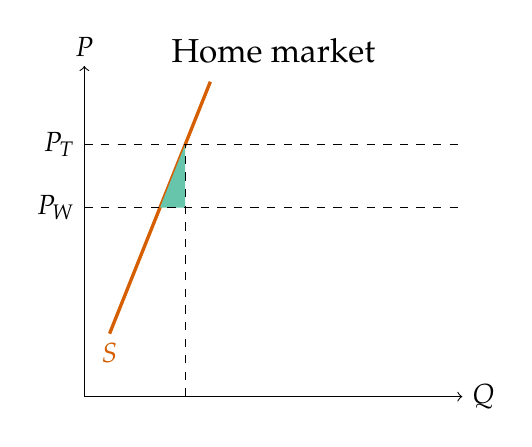
\begin{tikzpicture}[scale=0.4]

%---------------------------------------
% Shared functions
%---------------------------------------
\pgfmathdeclarefunction{QdH}{1}{\pgfmathparse{10 - 0.6*#1}}  % Home D
\pgfmathdeclarefunction{QsH}{1}{\pgfmathparse{0.4*#1}}       % Home S
\pgfmathdeclarefunction{QdF}{1}{\pgfmathparse{8 - 0.4*#1}}   % Foreign D*
\pgfmathdeclarefunction{QsF}{1}{\pgfmathparse{6 + 0.6*#1}}   % Foreign S*
\pgfmathdeclarefunction{MD}{1}{\pgfmathparse{10 - #1}}       % MD
\pgfmathdeclarefunction{XS}{1}{\pgfmathparse{6}}        % XS

\def\Pmin{2}
\def\Pmax{10}

% World equilibrium & tariff
\def\Pw{6}
\def\Qw{4}

\def\PT{8}
\def\Qt{{MD(\PT)}}
\def\twedge{2}

%====================================================
% LEFT PANEL: Home market
%====================================================
\begin{scope}[xshift=0cm]
  \node at (6,\Pmax+1) {\large Home market};

  % Axes
  \draw[->] (0,0) -- (0,\Pmax+0.5) node[above] {$P$};
  \draw[->] (0,0) -- (12,0) node[right] {$Q$};

  % Home demand and supply (true functional forms)

  \draw[very thick, red, domain=\Pmin:\Pmax, samples=100]
        plot ({QsH(\x)},{\x});

  \node[below, red]  at ({QsH(\Pmin)},\Pmin) {$S$};


  % ---- Tax Deadweight Loss ----
  \fill[green!60, opacity=1]
    ({QsH(\PT)},\PT)
    -- ({QsH(\PT)},\Pw)
    -- ({QsH(\Pw)},\Pw)
    -- cycle;

    
  \draw[dashed] ({QsH(\PT)},0) -- ({QsH(\PT)},\PT);
  % Prices PW and PT
  \draw[dashed] (0,\Pw) -- (12,\Pw);
  \draw[dashed] (0,\PT) -- (12,\PT);

  \node[left] at (0,\Pw) {$P_W$};
  \node[left] at (0,\PT) {$P_T$};
\end{scope}



\end{tikzpicture}
\end{figure}

\begin{itemize}
    \item The deadweight loss under the supply curve represents the domestic production distortion from the tariff
    \item Each additional unit of output is produced at a marginal cost above its opportunity cost (the world price $P_W$)
\end{itemize}

\end{frame}

\begin{frame}{Unpacking the deadweigth loss: consumption}
\addtocounter{framenumber}{-1}
\begin{figure}
\centering
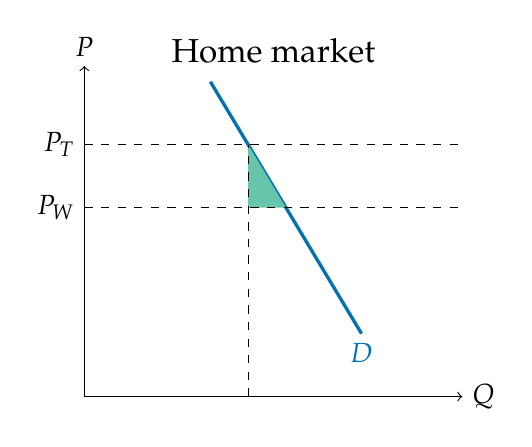
\begin{tikzpicture}[scale=0.4]

%---------------------------------------
% Shared functions
%---------------------------------------
\pgfmathdeclarefunction{QdH}{1}{\pgfmathparse{10 - 0.6*#1}}  % Home D
\pgfmathdeclarefunction{QsH}{1}{\pgfmathparse{0.4*#1}}       % Home S
\pgfmathdeclarefunction{QdF}{1}{\pgfmathparse{8 - 0.4*#1}}   % Foreign D*
\pgfmathdeclarefunction{QsF}{1}{\pgfmathparse{6 + 0.6*#1}}   % Foreign S*
\pgfmathdeclarefunction{MD}{1}{\pgfmathparse{10 - #1}}       % MD
\pgfmathdeclarefunction{XS}{1}{\pgfmathparse{6}}        % XS

\def\Pmin{2}
\def\Pmax{10}

% World equilibrium & tariff
\def\Pw{6}
\def\Qw{4}

\def\PT{8}
\def\Qt{{MD(\PT)}}
\def\twedge{2}

%====================================================
% LEFT PANEL: Home market
%====================================================
\begin{scope}[xshift=0cm]
  \node at (6,\Pmax+1) {\large Home market};

  % Axes
  \draw[->] (0,0) -- (0,\Pmax+0.5) node[above] {$P$};
  \draw[->] (0,0) -- (12,0) node[right] {$Q$};

  % Home demand and supply (true functional forms)
  \draw[very thick, blue, domain=\Pmin:\Pmax, samples=100]
        plot ({QdH(\x)},{\x});

  \node[below, blue] at ({QdH(\Pmin)},\Pmin) {$D$};
  

  % ---- Tax Deadweight Loss ----

   \fill[green!60, opacity=1]
    ({QdH(\PT)},\PT)
    -- ({QdH(\PT)},\Pw)
    -- ({QdH(\Pw)},\Pw)
    -- cycle;
    
  \draw[dashed] ({QdH(\PT)},0) -- ({QdH(\PT)},\PT);

  % Prices PW and PT
  \draw[dashed] (0,\Pw) -- (12,\Pw);
  \draw[dashed] (0,\PT) -- (12,\PT);

  \node[left] at (0,\Pw) {$P_W$};
  \node[left] at (0,\PT) {$P_T$};
\end{scope}



\end{tikzpicture}
\end{figure}
\begin{itemize}
    \item The deadweight loss under the demand curve represents the domestic consumption distortion from the tariff
    \item The marginal benefit of the foregone units consumption are above their opportunity cost (the world price $P_W$)
\end{itemize}
\end{frame}



\begin{frame}{Effects of a Tariff in a large country}
\begin{figure}
\centering
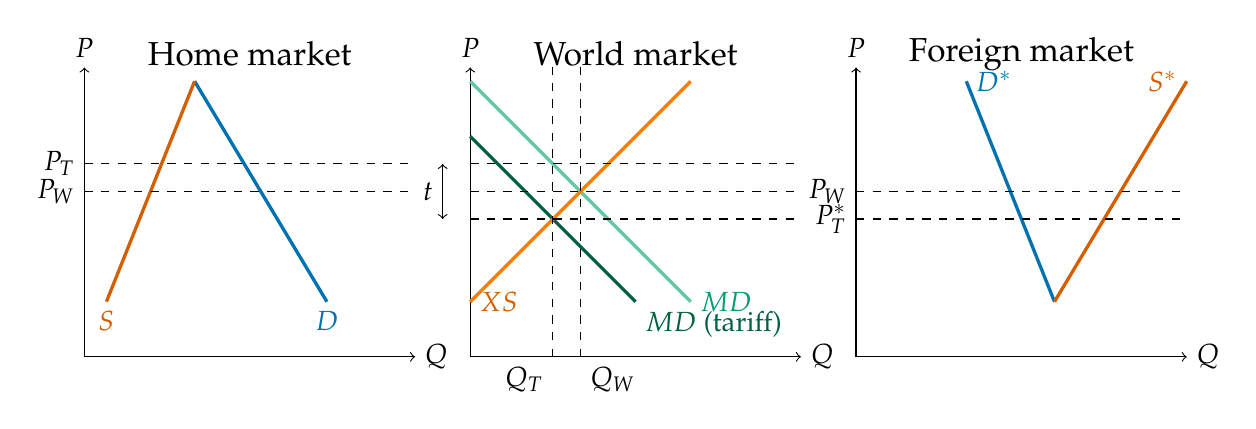
\begin{tikzpicture}[scale=0.35]

%---------------------------------------
% Shared functions
%---------------------------------------
\pgfmathdeclarefunction{QdH}{1}{\pgfmathparse{10 - 0.6*#1}}  % Home D
\pgfmathdeclarefunction{QsH}{1}{\pgfmathparse{0.4*#1}}       % Home S
\pgfmathdeclarefunction{QdF}{1}{\pgfmathparse{8 - 0.4*#1}}   % Foreign D*
\pgfmathdeclarefunction{QsF}{1}{\pgfmathparse{6 + 0.6*#1}}   % Foreign S*
\pgfmathdeclarefunction{MD}{1}{\pgfmathparse{10 - #1}}       % MD
\pgfmathdeclarefunction{MDt}{1}{\pgfmathparse{8 - #1}}       % MD
\pgfmathdeclarefunction{XS}{1}{\pgfmathparse{#1 - 2}}        % XS

\def\Pmin{2}
\def\Pmax{10}

% World equilibrium & tariff
\def\Pw{6}
\def\Qw{4}

\def\Qt{3}
\def\PT{7}
\def\PTstar{5}
\def\twedge{2}

%====================================================
% LEFT PANEL: Home market
%====================================================
\begin{scope}[xshift=0cm]
  \node at (6,\Pmax+1) {\large Home market};

  % Axes
  \draw[->] (0,0) -- (0,\Pmax+0.5) node[above] {$P$};
  \draw[->] (0,0) -- (12,0) node[right] {$Q$};

  % Home demand and supply (true functional forms)
  \draw[very thick, blue, domain=\Pmin:\Pmax, samples=100]
        plot ({QdH(\x)},{\x});
  \draw[very thick, red, domain=\Pmin:\Pmax, samples=100]
        plot ({QsH(\x)},{\x});

  \node[below, blue] at ({QdH(\Pmin)},\Pmin) {$D$};
  \node[below, red]  at ({QsH(\Pmin)},\Pmin) {$S$};

  % Prices PW and PT
  \draw[dashed] (0,\Pw) -- (12,\Pw);
  \draw[dashed] (0,\PT) -- (12,\PT);

  \node[left] at (0,\Pw) {$P_W$};
  \node[left] at (0,\PT) {$P_T$};
\end{scope}

%====================================================
% MIDDLE PANEL: World market (MD and XS)
%====================================================
\begin{scope}[xshift=14cm]
  \node at (6,\Pmax+1) {\large World market};

  % Axes
  \draw[->] (0,0) -- (0,\Pmax+0.5) node[above] {$P$};
  \draw[->] (0,0) -- (12,0) node[right] {$Q$};

  % MD and XS
  \draw[very thick, green!60, domain=\Pmin:\Pmax, samples=100]
      plot ({MD(\x)},{\x});
  \node[right, green] at ({MD(\Pmin)},{\Pmin}) {$MD$};
  \draw[very thick, green!60!black, domain=\Pmin:\Pmax-2, samples=100]
      plot ({MDt(\x)},{\x});
  \node[below right, green!60!black] at ({MDt(\Pmin)},{\Pmin}) {$MD$ (tariff)};
   \draw[very thick, orange, domain=\Pmin:\Pmax, samples=100]
      plot ({XS(\x)},{\x});
  \node[right, red] at ({XS(\Pmin)},{\Pmin}) {$XS$};

  % New quantity with tariff Q_T
  \draw[dashed] (\Qt,0) -- (\Qt,\Pmax+0.5);
  \node[below left] at (\Qt,0) {$Q_T$};



  % Vertical line at Q_W
  \draw[dashed] (\Qw,0) -- (\Qw,\Pmax+0.5);
  \node[below right] at (\Qw,0) {$Q_W$};

  % Horizontal lines for P_T, P_W, P_T^*
  \draw[dashed] (0,\Pw) -- (12,\Pw);
  \draw[dashed] (0,\PT) -- (12,\PT);
  \draw[dashed] (0,\PTstar) -- (12,\PTstar);

  % Tariff wedge t = P_T - P_T^*
  \draw[<->] (-1,\PT) -- (-1,\PTstar)
      node[midway,left] {$t$};
\end{scope}

%====================================================
% RIGHT PANEL: Foreign market
%====================================================
\begin{scope}[xshift=28cm]
  \node at (6,\Pmax+1) {\large Foreign market};

  % Axes
  \draw[->] (0,0) -- (0,\Pmax+0.5) node[above] {$P$};
  \draw[->] (0,0) -- (12,0) node[right] {$Q$};

  % Foreign demand and supply
  \draw[very thick, blue, domain=\Pmin:\Pmax, samples=100]
        plot ({QdF(\x)},{\x});
  \draw[very thick, red, domain=\Pmin:\Pmax, samples=100]
        plot ({QsF(\x)},{\x});

  \node[right, blue] at ({QdF(\Pmax)},\Pmax) {$D^*$};
  \node[left, red]  at ({QsF(\Pmax)},\Pmax) {$S^*$};

  % Prices P_W and P_T^*
  \draw[dashed] (0,\Pw) -- (12,\Pw);
  \draw[dashed] (0,\PTstar) -- (12,\PTstar);

  \node[left] at (0,\Pw) {$P_W$};
  \node[left] at (0,\PTstar) {$P_T^*$};
\end{scope}

\end{tikzpicture}
\end{figure}

\end{frame}


\begin{frame}{Effects of a Tariff in a large country: discussion}
\begin{wideitemize}
    \item In a large country, \blue{domestic import demand impacts global markets}

    \item<2-> World price $P_W$ not only typically taken as given (relax later), but \blue{affected by import demand}

    \item<3-> \textcolor{brown}{Export supply curve (XS)} is upward sloping

    \item<4-> Tariff decreases import prices to $P_T^*$ from the free trade equilibrium $P_W$ 
    \begin{itemize}
        \item we call this the terms of trade effect
        \item potentially, the tariff increase could be larger than the deadweight loss
        \item but consumers still lose (without redistribution)
        \item and only holds if country is large for given product market
    \end{itemize}
    \item<5-> In that case, prices increase less than the value of the tariff: $P = P_T^* + t < P_W + t $

    \item<6-> It will reduce imports to $Q_T< Q_W$
\end{wideitemize}
\end{frame}


\begin{frame}{Welfare effects of a Tariff in a large country}
\begin{figure}
\centering
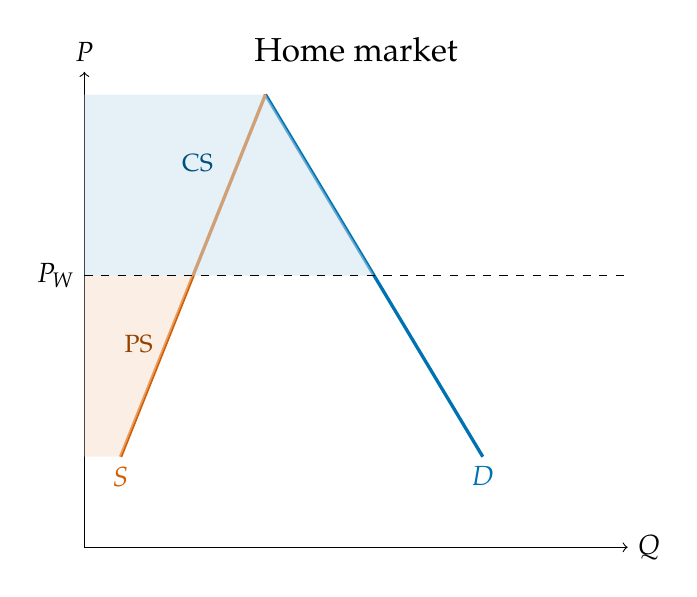
\begin{tikzpicture}[scale=0.575]

%---------------------------------------
% Shared functions
%---------------------------------------
\pgfmathdeclarefunction{QdH}{1}{\pgfmathparse{10 - 0.6*#1}}  % Home D
\pgfmathdeclarefunction{QsH}{1}{\pgfmathparse{0.4*#1}}       % Home S
\pgfmathdeclarefunction{QdF}{1}{\pgfmathparse{8 - 0.4*#1}}   % Foreign D*
\pgfmathdeclarefunction{QsF}{1}{\pgfmathparse{6 + 0.6*#1}}   % Foreign S*
\pgfmathdeclarefunction{MD}{1}{\pgfmathparse{10 - #1}}       % MD
\pgfmathdeclarefunction{XS}{1}{\pgfmathparse{6}}             % XS

\def\Pmin{2}
\def\Pmax{10}

% World equilibrium & tariff
\def\Pw{6}
\def\Qw{4}

\def\PT{8}
\def\Qt{{MD(\PT)}}
\def\twedge{2}

%====================================================
% LEFT PANEL: Home market
%====================================================
\begin{scope}[xshift=0cm]
  \node at (6,\Pmax+1) {\large Home market};

  % Axes
  \draw[->] (0,0) -- (0,\Pmax+0.5) node[above] {$P$};
  \draw[->] (0,0) -- (12,0) node[right] {$Q$};

  % Home demand and supply (true functional forms)
  \draw[very thick, blue, domain=\Pmin:\Pmax, samples=100]
        plot ({QdH(\x)},{\x});
  \draw[very thick, red, domain=\Pmin:\Pmax, samples=100]
        plot ({QsH(\x)},{\x});

  \node[below, blue] at ({QdH(\Pmin)},\Pmin) {$D$};
  \node[below, red]  at ({QsH(\Pmin)},\Pmin) {$S$};

  % ---- Consumer surplus (under D, above P_W) ----
  \fill[blue!20, opacity=0.5]
    (0,\Pw)
    -- ({QdH(\Pw)},\Pw)
    -- ({QdH(\Pmax)},\Pmax)
    -- (0,\Pmax)
    -- cycle;

  % Label CS
  \node[blue!70!black] at (2.5,8.5) {\small CS};

  % ---- Producer surplus (above S, below P_W) ----
  \fill[red!20, opacity=0.5]
    (0,\Pmin)
    -- (0,\Pw)
    -- ({QsH(\Pw)},\Pw)
    -- ({QsH(\Pmin)},\Pmin)
    -- (0,\Pmin)
    -- cycle;

  % Label PS
  \node[red!70!black] at (1.2,4.5) {\small PS};

  % World price line P_W
  \draw[dashed] (0,\Pw) -- (12,\Pw);
  \node[left] at (0,\Pw) {$P_W$};

\end{scope}

\end{tikzpicture}
\end{figure}

\end{frame}

\begin{frame}{Welfare effects of a Tariff in a large country}
\addtocounter{framenumber}{-1}

\begin{figure}
\centering
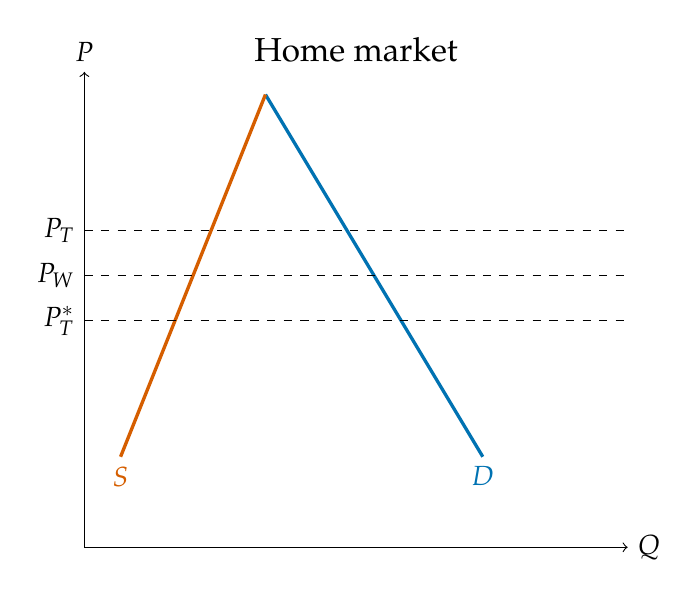
\begin{tikzpicture}[scale=0.575]

%---------------------------------------
% Shared functions
%---------------------------------------
\pgfmathdeclarefunction{QdH}{1}{\pgfmathparse{10 - 0.6*#1}}  % Home D
\pgfmathdeclarefunction{QsH}{1}{\pgfmathparse{0.4*#1}}       % Home S
\pgfmathdeclarefunction{QdF}{1}{\pgfmathparse{8 - 0.4*#1}}   % Foreign D*
\pgfmathdeclarefunction{QsF}{1}{\pgfmathparse{6 + 0.6*#1}}   % Foreign S*
\pgfmathdeclarefunction{MD}{1}{\pgfmathparse{10 - #1}}       % MD
\pgfmathdeclarefunction{XS}{1}{\pgfmathparse{6}}        % XS

\def\Pmin{2}
\def\Pmax{10}

% World equilibrium & tariff
\def\Pw{6}
\def\Qw{4}

\def\PT{7}
\def\PTstar{5}
\def\twedge{2}
\def\Qt{{MD(\PT)}}
\def\twedge{2}

%====================================================
% LEFT PANEL: Home market
%====================================================
\begin{scope}[xshift=0cm]
  \node at (6,\Pmax+1) {\large Home market};

  % Axes
  \draw[->] (0,0) -- (0,\Pmax+0.5) node[above] {$P$};
  \draw[->] (0,0) -- (12,0) node[right] {$Q$};

  % Home demand and supply (true functional forms)
  \draw[very thick, blue, domain=\Pmin:\Pmax, samples=100]
        plot ({QdH(\x)},{\x});
  \draw[very thick, red, domain=\Pmin:\Pmax, samples=100]
        plot ({QsH(\x)},{\x});

  \node[below, blue] at ({QdH(\Pmin)},\Pmin) {$D$};
  \node[below, red]  at ({QsH(\Pmin)},\Pmin) {$S$};

  % Prices PW and PT
  \draw[dashed] (0,\Pw) -- (12,\Pw);
  \draw[dashed] (0,\PT) -- (12,\PT);
  \draw[dashed] (0,\PTstar) -- (12,\PTstar);

  \node[left] at (0,\Pw) {$P_W$};
  \node[left] at (0,\PT) {$P_T$};
  \node[left] at (0,\PTstar) {$P_T^*$};
\end{scope}



\end{tikzpicture}
\end{figure}

\end{frame}

\begin{frame}{Welfare effects of a Tariff in a large country}
\addtocounter{framenumber}{-1}
\begin{figure}
\centering
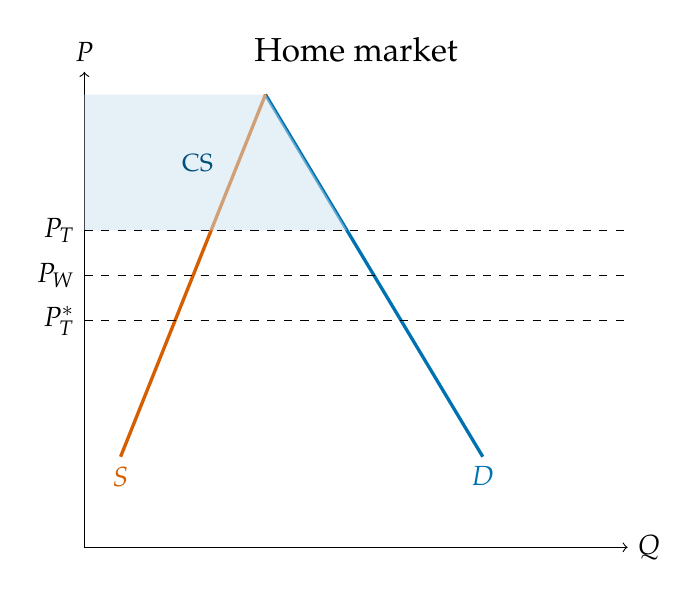
\begin{tikzpicture}[scale=0.575]


%---------------------------------------
% Shared functions
%---------------------------------------
\pgfmathdeclarefunction{QdH}{1}{\pgfmathparse{10 - 0.6*#1}}  % Home D
\pgfmathdeclarefunction{QsH}{1}{\pgfmathparse{0.4*#1}}       % Home S
\pgfmathdeclarefunction{QdF}{1}{\pgfmathparse{8 - 0.4*#1}}   % Foreign D*
\pgfmathdeclarefunction{QsF}{1}{\pgfmathparse{6 + 0.6*#1}}   % Foreign S*
\pgfmathdeclarefunction{MD}{1}{\pgfmathparse{10 - #1}}       % MD
\pgfmathdeclarefunction{XS}{1}{\pgfmathparse{6}}        % XS

\def\Pmin{2}
\def\Pmax{10}

% World equilibrium & tariff
\def\Pw{6}
\def\Qw{4}

\def\PT{7}
\def\PTstar{5}
\def\twedge{2}
\def\Qt{{MD(\PT)}}
\def\twedge{2}

%====================================================
% LEFT PANEL: Home market
%====================================================
\begin{scope}[xshift=0cm]
  \node at (6,\Pmax+1) {\large Home market};

  % Axes
  \draw[->] (0,0) -- (0,\Pmax+0.5) node[above] {$P$};
  \draw[->] (0,0) -- (12,0) node[right] {$Q$};

  % Home demand and supply (true functional forms)
  \draw[very thick, blue, domain=\Pmin:\Pmax, samples=100]
        plot ({QdH(\x)},{\x});
  \draw[very thick, red, domain=\Pmin:\Pmax, samples=100]
        plot ({QsH(\x)},{\x});

  \node[below, blue] at ({QdH(\Pmin)},\Pmin) {$D$};
  \node[below, red]  at ({QsH(\Pmin)},\Pmin) {$S$};

  % ---- Consumer surplus (under D, above P_W) ----
  \fill[blue!20, opacity=0.5]
    (0,\PT)
    -- ({QdH(\PT)},\PT)
    -- ({QdH(\Pmax)},\Pmax)
    -- (0,\Pmax)
    -- cycle;

  % Label CS
  \node[blue!70!black] at (2.5,8.5) {\small CS};


  % Prices PW and PT
  \draw[dashed] (0,\Pw) -- (12,\Pw);
  \draw[dashed] (0,\PT) -- (12,\PT);
  \draw[dashed] (0,\PTstar) -- (12,\PTstar);

  \node[left] at (0,\Pw) {$P_W$};
  \node[left] at (0,\PT) {$P_T$};
  \node[left] at (0,\PTstar) {$P_T^*$};
\end{scope}



\end{tikzpicture}
\end{figure}

\end{frame}


\begin{frame}{Welfare effects of a Tariff in a large country}
\addtocounter{framenumber}{-1}
\begin{figure}
\centering
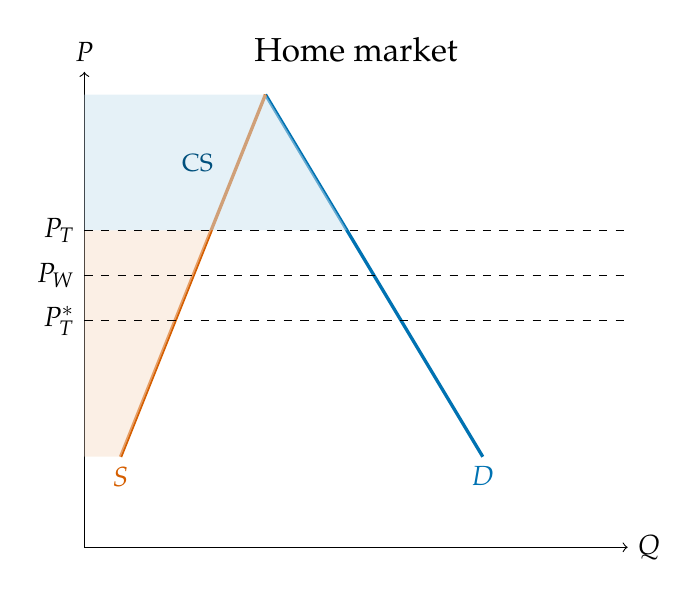
\begin{tikzpicture}[scale=0.575]

%---------------------------------------
% Shared functions
%---------------------------------------
\pgfmathdeclarefunction{QdH}{1}{\pgfmathparse{10 - 0.6*#1}}  % Home D
\pgfmathdeclarefunction{QsH}{1}{\pgfmathparse{0.4*#1}}       % Home S
\pgfmathdeclarefunction{QdF}{1}{\pgfmathparse{8 - 0.4*#1}}   % Foreign D*
\pgfmathdeclarefunction{QsF}{1}{\pgfmathparse{6 + 0.6*#1}}   % Foreign S*
\pgfmathdeclarefunction{MD}{1}{\pgfmathparse{10 - #1}}       % MD
\pgfmathdeclarefunction{XS}{1}{\pgfmathparse{6}}        % XS

\def\Pmin{2}
\def\Pmax{10}

% World equilibrium & tariff
\def\Pw{6}
\def\Qw{4}

\def\PT{7}
\def\PTstar{5}
\def\twedge{2}
\def\Qt{{MD(\PT)}}
\def\twedge{2}


%====================================================
% LEFT PANEL: Home market
%====================================================
\begin{scope}[xshift=0cm]
  \node at (6,\Pmax+1) {\large Home market};

  % Axes
  \draw[->] (0,0) -- (0,\Pmax+0.5) node[above] {$P$};
  \draw[->] (0,0) -- (12,0) node[right] {$Q$};

  % Home demand and supply (true functional forms)
  \draw[very thick, blue, domain=\Pmin:\Pmax, samples=100]
        plot ({QdH(\x)},{\x});
  \draw[very thick, red, domain=\Pmin:\Pmax, samples=100]
        plot ({QsH(\x)},{\x});

  \node[below, blue] at ({QdH(\Pmin)},\Pmin) {$D$};
  \node[below, red]  at ({QsH(\Pmin)},\Pmin) {$S$};

  % ---- Consumer surplus (under D, above P_W) ----
  \fill[blue!20, opacity=0.5]
    (0,\PT)
    -- ({QdH(\PT)},\PT)
    -- ({QdH(\Pmax)},\Pmax)
    -- (0,\Pmax)
    -- cycle;

  % Label CS
  \node[blue!70!black] at (2.5,8.5) {\small CS};

  % ---- Producer surplus (above S, below P_W) ----
  \fill[red!20, opacity=0.5]
    (0,\Pmin)
    -- (0,\PT)
    -- ({QsH(\PT)},\PT)
    -- ({QsH(\Pmin)},\Pmin)
    -- (0,\Pmin)
    -- cycle;

  % Prices PW and PT
  \draw[dashed] (0,\Pw) -- (12,\Pw);
  \draw[dashed] (0,\PT) -- (12,\PT);
  \draw[dashed] (0,\PTstar) -- (12,\PTstar);

  \node[left] at (0,\Pw) {$P_W$};
  \node[left] at (0,\PT) {$P_T$};
  \node[left] at (0,\PTstar) {$P_T^*$};
\end{scope}



\end{tikzpicture}
\end{figure}

\end{frame}



\begin{frame}{Welfare effects of a Tariff in a large country}
\addtocounter{framenumber}{-1}
\begin{figure}
\centering
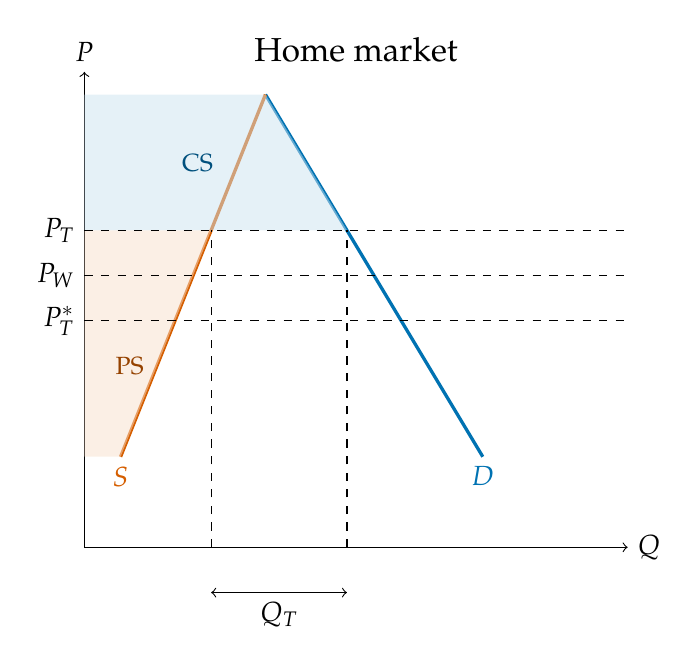
\begin{tikzpicture}[scale=0.575]

%---------------------------------------
% Shared functions
%---------------------------------------
\pgfmathdeclarefunction{QdH}{1}{\pgfmathparse{10 - 0.6*#1}}  % Home D
\pgfmathdeclarefunction{QsH}{1}{\pgfmathparse{0.4*#1}}       % Home S
\pgfmathdeclarefunction{QdF}{1}{\pgfmathparse{8 - 0.4*#1}}   % Foreign D*
\pgfmathdeclarefunction{QsF}{1}{\pgfmathparse{6 + 0.6*#1}}   % Foreign S*
\pgfmathdeclarefunction{MD}{1}{\pgfmathparse{10 - #1}}       % MD
\pgfmathdeclarefunction{XS}{1}{\pgfmathparse{6}}        % XS

\def\Pmin{2}
\def\Pmax{10}

% World equilibrium & tariff
\def\Pw{6}
\def\Qw{4}

\def\PT{7}
\def\PTstar{5}
\def\twedge{2}
\def\Qt{{MD(\PT)}}
\def\twedge{2}

%====================================================
% LEFT PANEL: Home market
%====================================================
\begin{scope}[xshift=0cm]
  \node at (6,\Pmax+1) {\large Home market};

  % Axes
  \draw[->] (0,0) -- (0,\Pmax+0.5) node[above] {$P$};
  \draw[->] (0,0) -- (12,0) node[right] {$Q$};

  % Home demand and supply (true functional forms)
  \draw[very thick, blue, domain=\Pmin:\Pmax, samples=100]
        plot ({QdH(\x)},{\x});
  \draw[very thick, red, domain=\Pmin:\Pmax, samples=100]
        plot ({QsH(\x)},{\x});

  \node[below, blue] at ({QdH(\Pmin)},\Pmin) {$D$};
  \node[below, red]  at ({QsH(\Pmin)},\Pmin) {$S$};

  % ---- Consumer surplus (under D, above P_W) ----
  \fill[blue!20, opacity=0.5]
    (0,\PT)
    -- ({QdH(\PT)},\PT)
    -- ({QdH(\Pmax)},\Pmax)
    -- (0,\Pmax)
    -- cycle;

  % Label CS
  \node[blue!70!black] at (2.5,8.5) {\small CS};

  % ---- Producer surplus (above S, below P_W) ----
  \fill[red!20, opacity=0.5]
    (0,\Pmin)
    -- (0,\PT)
    -- ({QsH(\PT)},\PT)
    -- ({QsH(\Pmin)},\Pmin)
    -- (0,\Pmin)
    -- cycle;

  % Label PS
  \node[red!70!black] at (1,4) {\small PS};

  \draw[dashed] ({QsH(\PT)},0) -- ({QsH(\PT)},\PT);
  \draw[dashed] ({QdH(\PT)},0) -- ({QdH(\PT)},\PT);
  \draw[<->] ({QsH(\PT)},-1) -- ({QdH(\PT)},-1)
      node[midway,below] {$Q_T$};
  % Prices PW and PT
  \draw[dashed] (0,\Pw) -- (12,\Pw);
  \draw[dashed] (0,\PT) -- (12,\PT);
  \draw[dashed] (0,\PTstar) -- (12,\PTstar);

  \node[left] at (0,\Pw) {$P_W$};
  \node[left] at (0,\PT) {$P_T$};
  \node[left] at (0,\PTstar) {$P_T^*$};
\end{scope}



\end{tikzpicture}
\end{figure}

\end{frame}


\begin{frame}{Welfare effects of a Tariff in a large country}
\addtocounter{framenumber}{-1}
\begin{figure}
\centering
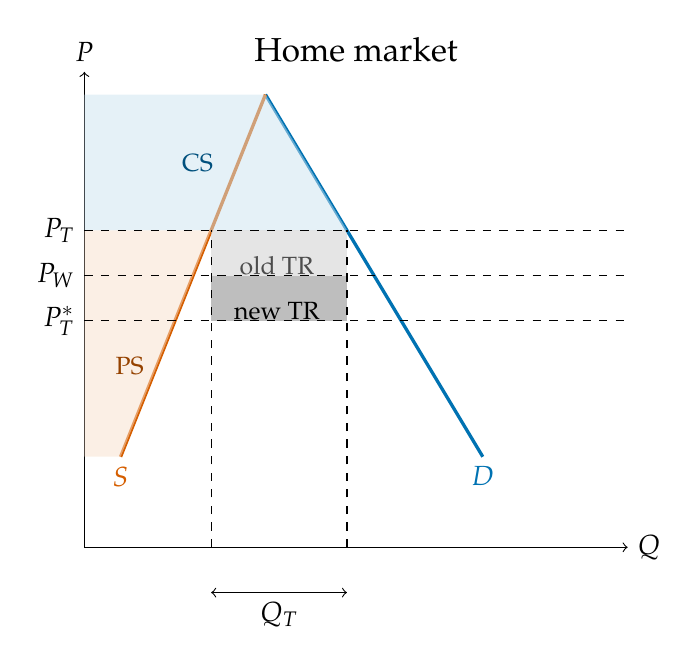
\begin{tikzpicture}[scale=0.575]

%---------------------------------------
% Shared functions
%---------------------------------------
\pgfmathdeclarefunction{QdH}{1}{\pgfmathparse{10 - 0.6*#1}}  % Home D
\pgfmathdeclarefunction{QsH}{1}{\pgfmathparse{0.4*#1}}       % Home S
\pgfmathdeclarefunction{QdF}{1}{\pgfmathparse{8 - 0.4*#1}}   % Foreign D*
\pgfmathdeclarefunction{QsF}{1}{\pgfmathparse{6 + 0.6*#1}}   % Foreign S*
\pgfmathdeclarefunction{MD}{1}{\pgfmathparse{10 - #1}}       % MD
\pgfmathdeclarefunction{XS}{1}{\pgfmathparse{6}}        % XS

\def\Pmin{2}
\def\Pmax{10}

% World equilibrium & tariff
\def\Pw{6}
\def\Qw{4}

\def\PT{7}
\def\PTstar{5}
\def\twedge{2}
\def\Qt{{MD(\PT)}}
\def\twedge{2}

%====================================================
% LEFT PANEL: Home market
%====================================================
\begin{scope}[xshift=0cm]
  \node at (6,\Pmax+1) {\large Home market};

  % Axes
  \draw[->] (0,0) -- (0,\Pmax+0.5) node[above] {$P$};
  \draw[->] (0,0) -- (12,0) node[right] {$Q$};

  % Home demand and supply (true functional forms)
  \draw[very thick, blue, domain=\Pmin:\Pmax, samples=100]
        plot ({QdH(\x)},{\x});
  \draw[very thick, red, domain=\Pmin:\Pmax, samples=100]
        plot ({QsH(\x)},{\x});

  \node[below, blue] at ({QdH(\Pmin)},\Pmin) {$D$};
  \node[below, red]  at ({QsH(\Pmin)},\Pmin) {$S$};

  % ---- Consumer surplus (under D, above P_W) ----
  \fill[blue!20, opacity=0.5]
    (0,\PT)
    -- ({QdH(\PT)},\PT)
    -- ({QdH(\Pmax)},\Pmax)
    -- (0,\Pmax)
    -- cycle;

  % Label CS
  \node[blue!70!black] at (2.5,8.5) {\small CS};

  % ---- Producer surplus (above S, below P_W) ----
  \fill[red!20, opacity=0.5]
    (0,\Pmin)
    -- (0,\PT)
    -- ({QsH(\PT)},\PT)
    -- ({QsH(\Pmin)},\Pmin)
    -- (0,\Pmin)
    -- cycle;

  % Label TR

  % ---- Tax Revenue ----
  \fill[black!20, opacity=0.5]
    ({QsH(\PT)},\PT)
    -- ({QdH(\PT)},\PT)
    -- ({QdH(\PT)},\PTstar)
    -- ({QsH(\PT)},\PTstar)
    -- cycle;

  \fill[black!30, opacity=.75]
    ({QsH(\PT)},\Pw)
    -- ({QdH(\PT)},\Pw)
    -- ({QdH(\PT)},\PTstar)
    -- ({QsH(\PT)},\PTstar)
    -- cycle;

  \node[black!70] at (4.25,6.225) {\small old TR};
  \node[black] at (4.25,5.225) {\small new TR};
    
  % Label PS
  \node[red!70!black] at (1,4) {\small PS};

  \draw[dashed] ({QsH(\PT)},0) -- ({QsH(\PT)},\PT);
  \draw[dashed] ({QdH(\PT)},0) -- ({QdH(\PT)},\PT);
  \draw[<->] ({QsH(\PT)},-1) -- ({QdH(\PT)},-1)
      node[midway,below] {$Q_T$};
  % Prices PW and PT
  \draw[dashed] (0,\Pw) -- (12,\Pw);
  \draw[dashed] (0,\PT) -- (12,\PT);
  \draw[dashed] (0,\PTstar) -- (12,\PTstar);

  \node[left] at (0,\Pw) {$P_W$};
  \node[left] at (0,\PT) {$P_T$};
  \node[left] at (0,\PTstar) {$P_T^*$};
\end{scope}



\end{tikzpicture}
\end{figure}

\end{frame}

\begin{frame}{Welfare effects of a Tariff in a large country}
\addtocounter{framenumber}{-1}
\begin{figure}
\centering
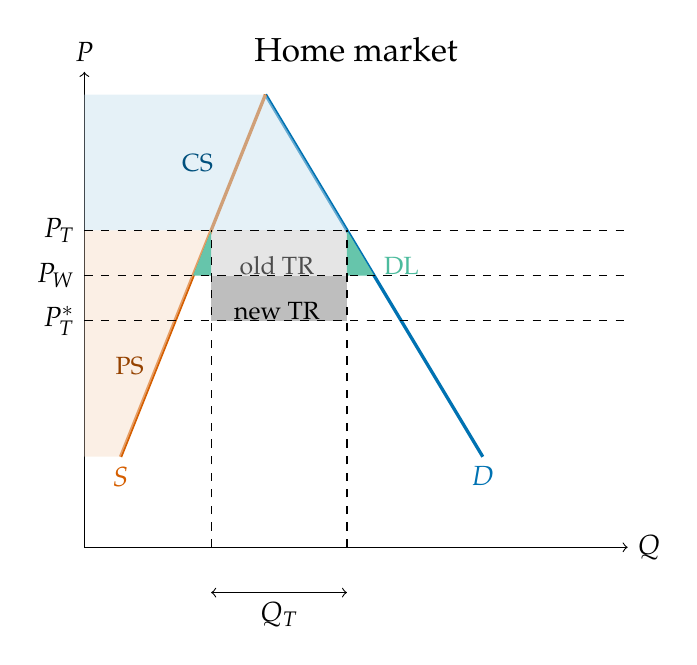
\begin{tikzpicture}[scale=0.575]

%---------------------------------------
% Shared functions
%---------------------------------------
\pgfmathdeclarefunction{QdH}{1}{\pgfmathparse{10 - 0.6*#1}}  % Home D
\pgfmathdeclarefunction{QsH}{1}{\pgfmathparse{0.4*#1}}       % Home S
\pgfmathdeclarefunction{QdF}{1}{\pgfmathparse{8 - 0.4*#1}}   % Foreign D*
\pgfmathdeclarefunction{QsF}{1}{\pgfmathparse{6 + 0.6*#1}}   % Foreign S*
\pgfmathdeclarefunction{MD}{1}{\pgfmathparse{10 - #1}}       % MD
\pgfmathdeclarefunction{XS}{1}{\pgfmathparse{6}}        % XS

\def\Pmin{2}
\def\Pmax{10}

% World equilibrium & tariff
\def\Pw{6}
\def\Qw{4}

\def\PT{7}
\def\PTstar{5}
\def\twedge{2}
\def\Qt{{MD(\PT)}}
\def\twedge{2}

%====================================================
% LEFT PANEL: Home market
%====================================================
\begin{scope}[xshift=0cm]
  \node at (6,\Pmax+1) {\large Home market};

  % Axes
  \draw[->] (0,0) -- (0,\Pmax+0.5) node[above] {$P$};
  \draw[->] (0,0) -- (12,0) node[right] {$Q$};

  % Home demand and supply (true functional forms)
  \draw[very thick, blue, domain=\Pmin:\Pmax, samples=100]
        plot ({QdH(\x)},{\x});
  \draw[very thick, red, domain=\Pmin:\Pmax, samples=100]
        plot ({QsH(\x)},{\x});

  \node[below, blue] at ({QdH(\Pmin)},\Pmin) {$D$};
  \node[below, red]  at ({QsH(\Pmin)},\Pmin) {$S$};

  % ---- Consumer surplus (under D, above P_W) ----
  \fill[blue!20, opacity=0.5]
    (0,\PT)
    -- ({QdH(\PT)},\PT)
    -- ({QdH(\Pmax)},\Pmax)
    -- (0,\Pmax)
    -- cycle;

  % Label CS
  \node[blue!70!black] at (2.5,8.5) {\small CS};

  % ---- Producer surplus (above S, below P_W) ----
  \fill[red!20, opacity=0.5]
    (0,\Pmin)
    -- (0,\PT)
    -- ({QsH(\PT)},\PT)
    -- ({QsH(\Pmin)},\Pmin)
    -- (0,\Pmin)
    -- cycle;

  % Label TR

  % ---- Tax Revenue ----
  \fill[black!20, opacity=0.5]
    ({QsH(\PT)},\PT)
    -- ({QdH(\PT)},\PT)
    -- ({QdH(\PT)},\PTstar)
    -- ({QsH(\PT)},\PTstar)
    -- cycle;

  \fill[black!30, opacity=.75]
    ({QsH(\PT)},\Pw)
    -- ({QdH(\PT)},\Pw)
    -- ({QdH(\PT)},\PTstar)
    -- ({QsH(\PT)},\PTstar)
    -- cycle;

  \node[black!70] at (4.25,6.225) {\small old TR};
  \node[black] at (4.25,5.225) {\small new TR};


  % Label DL
  \node[green!70] at (7,6.225) {\small DL};

  % ---- Tax Deadweight Loss ----
  \fill[green!60, opacity=1]
    ({QsH(\PT)},\PT)
    -- ({QsH(\PT)},\Pw)
    -- ({QsH(\Pw)},\Pw)
    -- cycle;

   \fill[green!60, opacity=1]
    ({QdH(\PT)},\PT)
    -- ({QdH(\PT)},\Pw)
    -- ({QdH(\Pw)},\Pw)
    -- cycle;
    
  % Label PS
  \node[red!70!black] at (1,4) {\small PS};

  \draw[dashed] ({QsH(\PT)},0) -- ({QsH(\PT)},\PT);
  \draw[dashed] ({QdH(\PT)},0) -- ({QdH(\PT)},\PT);
  \draw[<->] ({QsH(\PT)},-1) -- ({QdH(\PT)},-1)
      node[midway,below] {$Q_T$};
  % Prices PW and PT
  \draw[dashed] (0,\Pw) -- (12,\Pw);
  \draw[dashed] (0,\PT) -- (12,\PT);
  \draw[dashed] (0,\PTstar) -- (12,\PTstar);

  \node[left] at (0,\Pw) {$P_W$};
  \node[left] at (0,\PT) {$P_T$};
  \node[left] at (0,\PTstar) {$P_T^*$};
\end{scope}



\end{tikzpicture}
\end{figure}

\end{frame}


\begin{frame}{Welfare effects of a Tariff in a large country}
\addtocounter{framenumber}{-1}
\begin{figure}
\centering
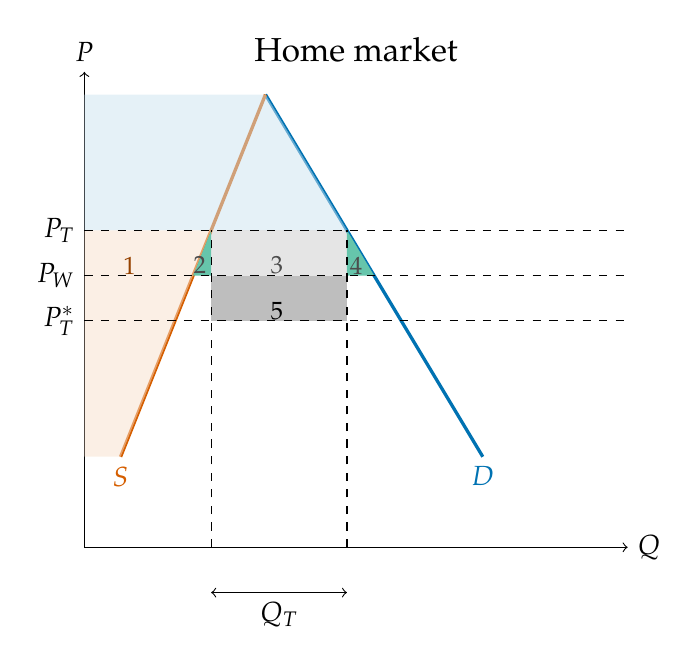
\begin{tikzpicture}[scale=0.575]

%---------------------------------------
% Shared functions
%---------------------------------------
\pgfmathdeclarefunction{QdH}{1}{\pgfmathparse{10 - 0.6*#1}}  % Home D
\pgfmathdeclarefunction{QsH}{1}{\pgfmathparse{0.4*#1}}       % Home S
\pgfmathdeclarefunction{QdF}{1}{\pgfmathparse{8 - 0.4*#1}}   % Foreign D*
\pgfmathdeclarefunction{QsF}{1}{\pgfmathparse{6 + 0.6*#1}}   % Foreign S*
\pgfmathdeclarefunction{MD}{1}{\pgfmathparse{10 - #1}}       % MD
\pgfmathdeclarefunction{XS}{1}{\pgfmathparse{6}}        % XS

\def\Pmin{2}
\def\Pmax{10}

% World equilibrium & tariff
\def\Pw{6}
\def\Qw{4}

\def\PT{7}
\def\PTstar{5}
\def\twedge{2}
\def\Qt{{MD(\PT)}}
\def\twedge{2}

%====================================================
% LEFT PANEL: Home market
%====================================================
\begin{scope}[xshift=0cm]
  \node at (6,\Pmax+1) {\large Home market};

  % Axes
  \draw[->] (0,0) -- (0,\Pmax+0.5) node[above] {$P$};
  \draw[->] (0,0) -- (12,0) node[right] {$Q$};

  % Home demand and supply (true functional forms)
  \draw[very thick, blue, domain=\Pmin:\Pmax, samples=100]
        plot ({QdH(\x)},{\x});
  \draw[very thick, red, domain=\Pmin:\Pmax, samples=100]
        plot ({QsH(\x)},{\x});

  \node[below, blue] at ({QdH(\Pmin)},\Pmin) {$D$};
  \node[below, red]  at ({QsH(\Pmin)},\Pmin) {$S$};

  % ---- Consumer surplus (under D, above P_W) ----
  \fill[blue!20, opacity=0.5]
    (0,\PT)
    -- ({QdH(\PT)},\PT)
    -- ({QdH(\Pmax)},\Pmax)
    -- (0,\Pmax)
    -- cycle;

  % Label CS

  % ---- Producer surplus (above S, below P_W) ----
  \fill[red!20, opacity=0.5]
    (0,\Pmin)
    -- (0,\PT)
    -- ({QsH(\PT)},\PT)
    -- ({QsH(\Pmin)},\Pmin)
    -- (0,\Pmin)
    -- cycle;

  % Label TR

  % ---- Tax Revenue ----
  \fill[black!20, opacity=0.5]
    ({QsH(\PT)},\PT)
    -- ({QdH(\PT)},\PT)
    -- ({QdH(\PT)},\PTstar)
    -- ({QsH(\PT)},\PTstar)
    -- cycle;

  \fill[black!30, opacity=.75]
    ({QsH(\PT)},\Pw)
    -- ({QdH(\PT)},\Pw)
    -- ({QdH(\PT)},\PTstar)
    -- ({QsH(\PT)},\PTstar)
    -- cycle;

  \node[black!70] at (4.25,6.225) {\small 3};
  \node[black] at (4.25,5.225) {\small 5};




  % ---- Tax Deadweight Loss ----
  \fill[green!60, opacity=1]
    ({QsH(\PT)},\PT)
    -- ({QsH(\PT)},\Pw)
    -- ({QsH(\Pw)},\Pw)
    -- cycle;

   \fill[green!60, opacity=1]
    ({QdH(\PT)},\PT)
    -- ({QdH(\PT)},\Pw)
    -- ({QdH(\Pw)},\Pw)
    -- cycle;
    
  % Label PS
  \node[red!70!black] at (1,6.225) {\small 1};

  \draw[dashed] ({QsH(\PT)},0) -- ({QsH(\PT)},\PT);
  \draw[dashed] ({QdH(\PT)},0) -- ({QdH(\PT)},\PT);
  \draw[<->] ({QsH(\PT)},-1) -- ({QdH(\PT)},-1)
      node[midway,below] {$Q_T$};
  % Prices PW and PT
  \draw[dashed] (0,\Pw) -- (12,\Pw);
  \draw[dashed] (0,\PT) -- (12,\PT);
  \draw[dashed] (0,\PTstar) -- (12,\PTstar);

  \node[left] at (0,\Pw) {$P_W$};
  \node[left] at (0,\PT) {$P_T$};
  \node[left] at (0,\PTstar) {$P_T^*$};

  % Label DL
  \node[black!70] at (2.55,6.225) {\small 2};
  \node[black!70] at (6,6.225) {\small 4};
  
  \end{scope}



\end{tikzpicture}
\end{figure}

\end{frame}


\begin{frame}{New tariff revenue vs deadweight loss}
\begin{wideitemize}

    \item Tariff decreases import prices to $P_T^*$ from the free trade equilibrium $P_W$ 
    \item<2-> This means that deadweight loss is smaller, since $P = P_T^* + t < P_W + t $
    \item<3-> Whether the country is better off or worse off, it depends
    \item<4-> ``Old'' tariff revenue used to be CS, so it is a wash
    \item<5-> Tariff induces deadweight loss...
    \item<5-> ...but it also has an additional tariff revenue due to terms of trade effect
    \item<6-> So relevant question: is ``new'' tariff revenue larger/smaller than deadeweight loss?

    \end{wideitemize}
\end{frame}


\begin{frame}{Optimal tariffs}
\begin{itemize}

    \item For a large country, what are the net changes in welfare induced by a tariff? 
    \item Relative importance of the gain from the terms of trade improvement and the production/consumption distortions

    \begin{figure}
        \centering
        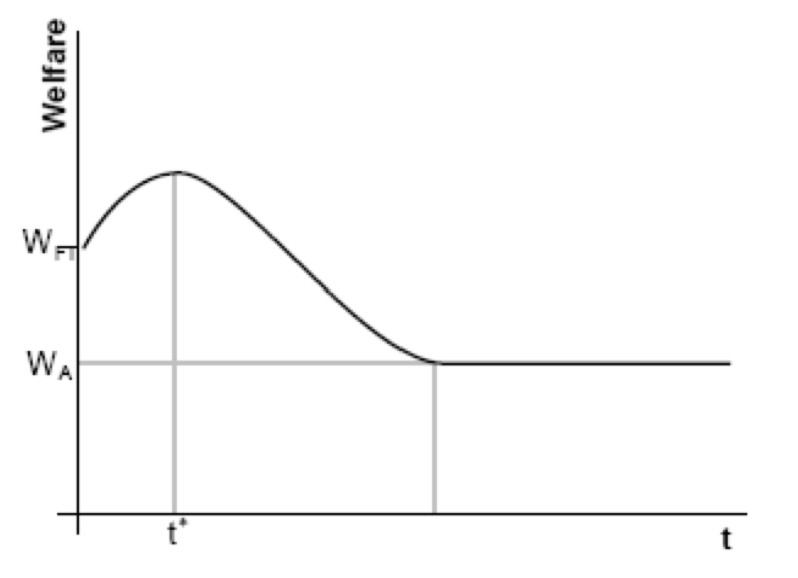
\includegraphics[width=0.45\linewidth]{figs/optimal-tariff.jpg}
    \end{figure}

    \item For small tariffs, the gain from the terms of trade improvement dominates, but not for larger tariffs $\implies$ there is an ‘optimal’ tariff level $t^*$
    \item  The more the foreign export supply to a country is inelastic, the higher the optimal tariff $t^*$
    \end{itemize}
\end{frame}

\end{document}
